% REMEMBER: You must not plagiarise anything in your report. Be extremely careful.

\documentclass{l4proj}

    
%
% put any additional packages here
%

\begin{document}

%==============================================================================
%% METADATA
\title{Imputation strategies for risk prediction models based on Electronic Health Records}
\author{Lee Lok Hang Toby}
\date{September 14, 2021}

\maketitle

%==============================================================================
%% ABSTRACT
\begin{abstract}


    The digitisation of health records in recent years created large amount of healthcare data that are now publicly available for researchers. Along side recent advancements in machine learning and artificial intelligence, accurate and robust clinical decision support systems using machine learning is made possible. However, Electronic Health Records (EHR) are complex and irregularly sampled, which introduces the problem of missing data. Previous researches often exclude patients with missing data in their dataset, which makes the population sample not representative and could introduce biases.
    
    Uni-variate imputation strategies like mean imputation is often used to solve this problem, but was proven to be ineffective and introduces bias to the clinical decision machine learning models in this research. 
    
    To conduct in-depth analysis on imputation strategies with electronic health records, the publicly available clinical database MIMIC-III is used. This dissertation includes detailed extraction pipeline to extract events and patient data, along side pre-processing steps so that it is ready for imputation and machine learning. Mean, most-frequent and knn imputation are common approaches for it's effectiveness and ease of implementation. This research dives deeper to apply advanced multiple imputation techniques featuring chained equations and denoising auto-encoders.After implementation, the imputed datasets are evaluated using leave one out cross validation (LOOCV) simulation and statistical performances of risk prediction model created to predict in-hospital mortality.
    
    It was found that Multiple imputation by chained equations (MICE) is the all-rounded winner by small margins over other imputation strategies both in terms of it's ability to impute data similar of the original, and evaluation metrics performances for the in-hospital mortality classifier. 
    
    
    
\end{abstract}

\pagebreak

\renewcommand{\abstractname}{Acknowledgements}
\begin{abstract}
    I would like to offer my deepest gratiude to Dr. Fani Deligianni for her excellence supervision during the course of my Honours project. With limited knowledge for this field of research, Dr. Deligianni offered detailed guidance and patient response to my countless questions. Throughout the course, Dr Deliganni offered weekly meetings for questions and offered constant support along side friendly encouragements. I am truly indebted to Dr. Deliganni for guiding me through this journey. 

\end{abstract}

    

%==============================================================================

% EDUCATION REUSE CONSENT FORM
% If you consent to your project being shown to future students for educational purposes
% then insert your name and the date below to  sign the education use form that appears in the front of the document. 
% You must explicitly give consent if you wish to do so.
% If you sign, your project may be included in the Hall of Fame if it scores particularly highly.
%
% Please note that you are under no obligation to sign 
% this declaration, but doing so would help future students.
%

\def\consentname {Lee Lok Hang Toby} % your full name
\def\consentdate {1st April 2022} % the date you agree
%
\educationalconsent


%==============================================================================
\tableofcontents

%==============================================================================
%% Notes on formatting
%==============================================================================
% The first page, abstract and table of contents are numbered using Roman numerals and are not
% included in the page count. 
%
% From now on pages are numbered
% using Arabic numerals. Therefore, immediately after the first call to \chapter we need the call
% \pagenumbering{arabic} and this should be called once only in the document. 
%
% Do not alter the bibliography style.
%
% The first Chapter should then be on page 1. You are allowed 40 pages for a 40 credit project and 30 pages for a 
% 20 credit report. This includes everything numbered in Arabic numerals (excluding front matter) up
% to but excluding the appendices and bibliography.
%
% You must not alter text size (it is currently 10pt) or alter margins or spacing.
%
%
%==================================================================================================================================
%
% IMPORTANT
% The chapter headings here are **suggestions**. You don't have to follow this model if
% it doesn't fit your project. Every project should have an introduction and conclusion,
% however. 
%
%==================================================================================================================================
\graphicspath{ {./images/} }

\chapter{Introduction}

Health records is the collection of patient's information, often including the patient's symptoms along side comments of the healthcare practitioner and medical recordings for past lab exams. Traditionally, health records were stored in a paper-based record system using physical means like paper, discs, and films. These data are then organised and stored within physical storage facilities and retrieved when needed. Since these records are stored physically across different healthcare providers, it is difficult to share these records for a more efficient healthcare service.  

Electronic Health records (EHR) is a systematized digital collection of patient's information. Early efforts in developing Eletronic health records between 1971 and 1992 introduces storing electronic health records with hierarchical and relational database \cite{Evans2016-bp}.  This allows more efficient storing and access over the traditional system. As technology advances, these system moved from large mainframe computers to minicomputers, requiring less and less physical space for storage. In the last decade, EHR has evolved in various ways and revolutionized the healthcare world. Efficient storing and extraction of health records is now possible with faster and smaller computers. Accurate, up to date, and complete information about patients are quickly accessible by different clinics, allowing a more coordinated healthcare system. The advances in cyber security also allow secure storing and sharing of these records, enhancing the privacy and security of patients data. Lastly, EHR now contains a more detailed medical history, including diagnoses, medications, treatment plans, immunization dates, allergies, radiology images, and laboratory and test results.

% reset page numbering. Don't remove this!
\pagenumbering{arabic} 


\section{Motivation}

Machine learning is a type of artificial intelligence that can be used to learn patterns from data and make predictions. It can also be used to create risk prediction models that could help in managing medical resources and improving healthcare services. However applications in clinical-decision support system is found to be very limited due to the challenges in summarizing and representing patient data, along side privacy concerns and ethical issues of using real patients data, \cite{AyalaSolares2020}.

Due to the digitisation of health records, large amount of healthcare data are easily accessible digitally, which introduces the possibility to share these records with researchers around the world for scientific purposes. Since electronic health records consists of private information including name, gender, date of birth, and other sensitive identification information, these electronic health records are often not publicly available. It is until recently, a large, publicly available, and deidentified clinical database named MIMIC-III is released, which allow researchers from different fields to get their hands on large amount detailed and organised clinical data.

 Despite the introduction to new data, one of the biggest problem of missing data in electronic health records still remains. Most clinical data are time series data with different measurements taken at different times, meaning there will be missing measurements in some time frame for each patient. These missing data are often not missing at random, meaning there is a meaning and reason to why this data is missing, which further complicates the problem. Missing data limits our ability to train the risk prediction model and reduces the statistical power of our model. To solve this problem, imputation strategies is applied to impute these missing data, and different approaches to this problem could greatly affect the performances of these risk decision models.


\section{Aims}

This research focuses on how to use imputation strategies to improve risk prediction models for clinical decision support systems. As summarising and pre-processing electronic health records is not trivial, this research guides the reader through extraction and pre-processing pipeline for patients and events data from the MIMIC-III database. Different imputation strategies will then be applied to the pre-processed clinical data, where the effectiveness of these strategies is analysed through evaluating the accuracy of the risk prediction model created. To further evaluate these imputation strategies, multiple statistical analysis is carried out including various descriptive visualisations and data sample holdout simulations. 

\section{Outline}
This chapter covered the motivation and aims of this research. \textbf{Chapter 2} explains the background theories used in this project. \textbf{Chapter 3} provides guidance to setup the research environment for recreating this research. \textbf{Chapter 4} guides the reader through the design logic and data extraction from the clinical database.\textbf{ Chapter 5} explains all the imputation strategies implemented and how the machine learning models are built. \textbf{Chapter 6} presents the results of the investigation  and evaluates the performance of these strategies. \textbf{Chapter 7} includes the discussion and conclusion of the project.


%==================================================================================================================================
\chapter{Background}

\section{Healthcare information Retrieval from Data}
We can conceptualize the health care information retrieval processes as a pathway from 3 different type of analytics: Descriptive, predictive and prescriptive. 

\subsection{Descriptive Analytics}
Descriptive analytics is a form of analytics that brings insight through analysing data from history. It uses techniques like data aggregation, data mining and intuitive visualisation to provide understanding of historic data, \cite{healthcareML}. Common examples of descriptive analytics are reports that answers questions for the number of admitted patients in the hospital last year, or the number of patients that died in within 48 hours in an ICU unit. These queries can then be represented using histograms or probabilistic distributions for better visualisation and analysis of the data. To achieve substantial results in descriptive Analytics with medical data, data linking can be further used to link different sources of data across different faculties. For example, linking all information related to a patient across different departments to better understand the entire clinical history of the patient. The limitations of descriptive analytics is it's limited ability to guide clinical decision since it is only based on snapshots of the past, which might not always be indicative of the what will happen in the future. 

\subsection{Diagnostic Analytics}
Diagnostic analytics is a form of analytics that examines the data to answer questions to why something happened. Using techniques such as data discovery and correlations, diagnostic analytics aims to find answers to the patterns and problems identified from descriptive analytics, \cite{healthcareML}. For example, after identifying patients that stayed more than 48 hours in ICU units has higher death rate using descriptive analytics, diagnostic analystics is used to find out the reason behind this higher death-rate by finding correlations in historical data.

\subsection{Predictive Analytics}
Predictive analytics is a form of analytics that exploit historic values of the data with the aim to provide useful information about critical events in the future. Predictive analytics tools are in demand as healthcare providers seek evidence-based ways to reduce cost and avoid penalites associated with failure to control chronic diseases and adverse events that are preventable, \cite{healthcareML}. This further suggest the importance of predictive anlytics in healthcare as it has the potential to save many patients lives and improve the quality of healthcare services.

Clinical decision support system an example of a predictive analytics tools that predicts the likelihood of an event and provide assistance in making decisions for optimal clinical outcomes. 

\subsection{Prescriptive Analytics}
Prescriptive analytics is a form of analytics that aims to make decisions for optimal outcomes. It uses all the valuable information extracted from previous analytics to come to a decision with relation to what action should be taken. While predictive analytics helps us to understand the impact of an intervention in clinical care, prescriptive analytics attempts to quantify the effect of this future decision, and provide advice for possible outcomes. In other words, prescriptive analytics transform a prediction model, into a decision making model.


\section{Missing Data in Electronic Health Records}

In electronic health records, missing data can occur due to various reasons. Some common factors include difficulty in measuring indicators, improper handling of data storage in the system, and untimely data collection by medical staff, \cite{Wang2022}.

An often strategy to handle these missing values without imputation is to discard the entire row or column containing a missing value. However this approach comes at the price of losing possible valuable data and introduce biases in the dataset. Another important concept is that missing data in electronic health records could be both intentional or unintentional. Certain laboratory tests might not be carried out for the patient because a similar test is already taken, or the patient simply does not need the test. This suggests the concept that the data is not missing at random, which is one of the three types of missing data in imputation study: \textbf{Missing at Random}, \textbf{Missing completely at random}, and \textbf{missing not at random}.

\subsection{Missing completely at Random (MCAR)}

Missing completely at random is when the probability of missing is the same for all cases, \cite{buuren_2021}. This implies that the causes of missing data are completely unrelated to the data. An example of MCAR could be because of sudden power shortage in the hospital, which caused the machines to temporally disconnect from the system and lost some measurements. While it is convenient to treat missing data as MCAR, the chances are relatively low and doing so might ignore useful information if it was actually Missing not at random (MNAR).

\subsection{Missing at Random }

Missing at random is when the probability of missing is the same only within groups defined by the observed data. This implies that the cause of the missing data is somewhat related to the data, but not directly. An example of MAR would could be because the patient has a surgery that day, therefore the regular measurements for heart rate and blood pressure is missing. Different from MCAR, MAR is a broader class and often more realistic, therefore modern missing methods generally start from the MAR assumption, \cite{buuren_2021}.


\subsection{Missing not at Random (MNAR)}

Missing not at random is when the probability of missing varies varies for reasons that are unknown. This implies that the cause of the missing the data is directly related to the data. An example of MNAR would be because the patient simply does not require this laboratory test for his symptoms, therefore was left empty. In a machine learning environment, Missing not at random introduces a lot of complexity since these missing values could carry hidden meaning that could be provide useful information. If these missing value is simply removed or ignored, it would introduce bias since we are ignoring information provided to us. This is another reason why more complex imputation strategies is used to try and preserve these meanings and reduce bias in our training environment.


\section{Risk prediction models on Electronic Health records}

A risk prediction model uses patient data to estimate the probability of a patient experiencing a healthcare outcome. The adoption of clinical risk prediction tools was great limited previously by lack of integration with electronic health records suggested by previous researches, \cite{Sharmae100253}. Other researches also mentioned the rigorous process of this task in nature, where problems such as incomplete training data and risk of bias fails to address clinical need. However, With the recent releases of publicly available clinical database, and advancement in both machine learning and imputation strategies, more accurate and reliable risk prediction models are now possible.

Since electronic health records are heterogeneous with all sorts of medical recordings, these recordings must be extracted carefully and reorganised for machine learning. Recent researches suggest the approach to arrange individual measurements in a time series manner. By arranging the medical data by rows of time series, the machine learning model is able to learn complex temporal patterns from the data and improve performance, \cite{Harutyunyan2019}. 

\subsection{In hospital mortality as a Clinical outcome}

Mortality is one of the most common and important clinical outcome used in risk prediction models. In this research, in-hospital mortality in ICU will be used as a benchmark task for comparing the effectiveness of our different imputation strategies. 

Risk of mortality is often formulated as a binary classification task, where 0 indicates the patient is still alive and 1 indicates the patient is deceased. In order to evaluate the performance of the risk prediction model, the predicted outcome is compared with the true outcome extracted from the clinical dataset. 

\subsection{Classification Models}
To perform the classification tasks in predicting in hospital mortality, three different classifiers from popular machine learning libary sci-kit learn is used as baselines to test and evaluate the performance, \cite{scikit-learn}. The three classification models are Logistic Regression, Random Forest, and Support Vector Classifier.


\section{Public Electronic Health Records Dataset - MIMIC III} 

In the last few decades, Electronic health records continued to grow in size and with more patient consenting their records for research purposes, it made publicly available electronic health record dataset possible. The EHR dataset used in this research is the MIMIC-III dataset, which is the third version of the MIMIC dataset.

\subsection{History of MIMIC Datasets}
    The first MIMIC database is published in 1999, it contains medical data recorded over 90 ICU patients with ECG signals recorded at 500 samples per second with 12-bit precision. In April 2011 a new version of the database named MIMIC-II is released. The highly used MIMIC-II v2.6 it contains 32536 subjects with 40426 ICU admissions. Compared to the previous version, MIMIC II documents a significantly larger population of intensive care units patients and includes physiological waveforms and minute-by-minute trends for a subset of records. This introduces a unique resource to critical care research and allowing a wider range of analytical studies spanning across multiple fields. \\
    Finally, MIMIC-III is an updated version of MIMIC II v2.6, a large, freely-available Clinical database with approximately sixty thousand admissions of over forty thousand patients who stayed in the critical care units of the Beth Israel Deaconess Medical Center between 2001 and 2012. The database includes demographics, vital signs measurements, laboratory test results, medications, procedures, imaging reports, care giver notes, and the in hospital mortality for these patient. \cite{PhysioNet_MIMIC-III}. 
    
    
    Although the database is unidentified, it still contains detailed information of patients from the clinical care unit, therefore must be treated with appropriate care and respect. Researchers are often required to request access and complete a ethics course before being able to access the database.
    
    
\subsection{MIMIC-III as a relational Database}
    Since the data in MIMIC-III is collected from a hospital, schema and structure of the database closely resembles how the data is stored in the original source. Only small adjustments has been made to take into considerations how the users of the database could perform query and extract these data efficiently.

    There are a total of 26 tables in the MIMIC-III relational Database, which can be categorized into 4 different sections, \textbf{Patient Tracking}, \textbf{ICU Data}, \textbf{Hospital Data}, and \textbf{Dictionary Tables}:

    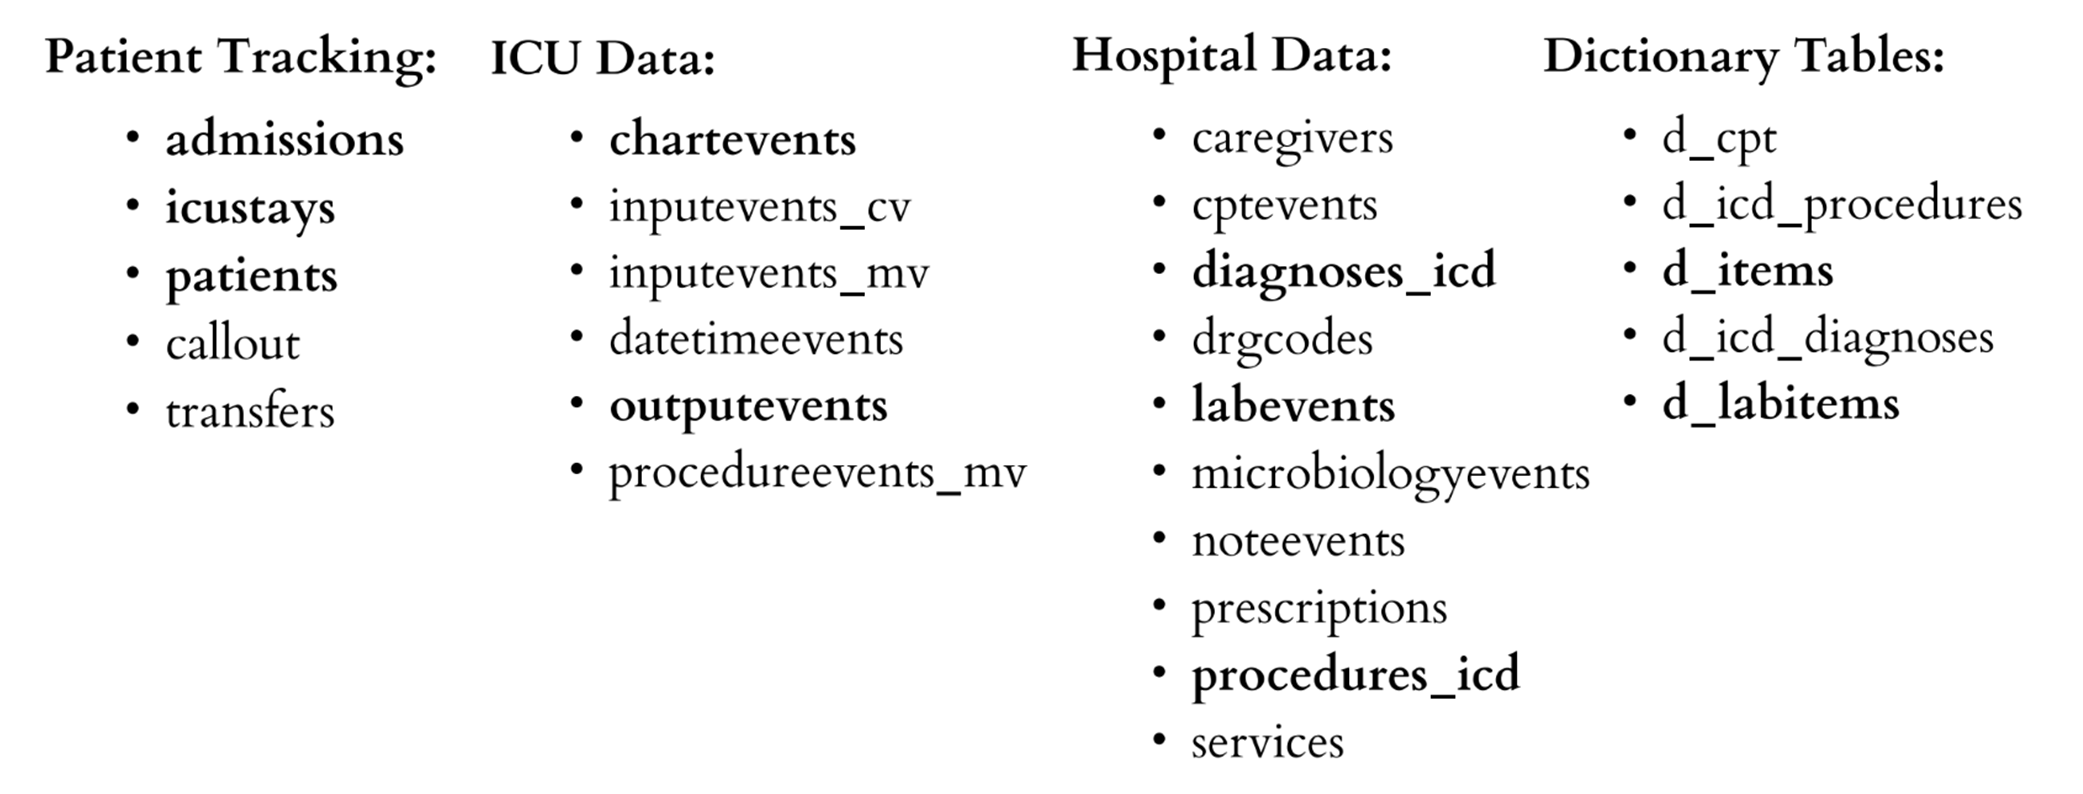
\includegraphics[width=\textwidth]{dissertation/Latex/images/tables.PNG}
        
    Tables in the \textbf{Patient Tracking} section is used to define and track patient stay. The first table used in this category is the \textbf{patients} table, since the database is unidentified, there are no patient names in this table, however, basic identification data like date of birth and gender is still stored. The second table used is the \textbf{admissions} table, where data regrading each admission is stored. Admission details includes the admission time, discharge time, death time, diagnosis, etc. The admission time and discharge time is used to calculate the length of stay of a patient in the hospital, which could be used to perform cohort selection later. The last table is the \textbf{icustays} table, this table connects each patient to it's ICU data using icustay\verb|_|id, and stores all the administrative patient information rather than the actual medical recordings. The one thing in common for these three table used is the subject|\verb|_||id attribute, where it is used to extract and combine hamd\verb|_|id (hospital admission id) from admissions table and icustay\verb|_|id from icustay table, which acts as the core indexing system for the dataframe in this project.

    Tables in the \textbf{ICU Data} section stores all the medical recordings for patients the entered the ICU. The only but most important table used in this category is the \textbf{chartevents} table. Chartevents is the largest table in the MIMIC-III dataset and is where most of the medical readings are stored. Each event in the table is a measurement of a patient labelled with the time it is recorded and stored by the medical staff. Each event has a value, the unit of this value, and the type of measurement indicated by an item id. 
    
   Tables in the \textbf{Hospital Data} section is stores all the medical recordings for patients in the hospital, which is separate from the ICU data. The table used from this category is the \textbf{labevents} table. Similar to chartevents, lab event stores all the lab data recordings with it's recorded time, value, units, and itemid to identify what type of lab recording it is.
     
    Tables in the \textbf{Dictionary Table} section stores mapping details for each hospital item to it's corresponding fields. the \textbf{d}\verb|_|\textbf{items} and \textbf{d}\verb|_|\textbf{labitems} table is used for chartevents and labevents correspondingly to extract the name given its item id. In this project, a resource file itemid\verb|_|to\verb|_|variable\verb|_|map.csv from https://github.com/MLforHealth/MIMIC\verb|_|Extract is used for ease of implementation. 


%==================================================================================================================================
\chapter{Analysis/Requirements}

\section{Project Aims}

The original aim of the project was to simply develop machine learning models to process electronic health record. However, the deep learning models implemented failed to further improve the results of the risk prediction model significantly. Therefore the project further developed into a deep dive for different imputation strategies to solve the ambiguous problem of missing data in electronic health records. This research aimed to come to a conclusion if deep learning imputation strategies is capable of out-performing state-of the art multiple imputations methods along side multiple baselines for a fair evaluation.

\section{Functional Requirements}
\subsection{Must have}
\begin{itemize}
  \item Explore the MIMIC-III and form appropriate queries to extract medical variables based on specific exclusion/inclusion criteria.
  \item Pre-process the medical variables to convert units, remove outliers and reorganise the data into time series of 48 hours for each patient.
  \item Use different imputation strategies to impute missing values found in the time series data
  \item Create Risk prediction models using different imputation strategy
  \item Evaluate the performance of risk prediction models with different imputation strategies.

\end{itemize}

\subsection{Should have}

\begin{itemize}
  \item Exploit Deep Learning approaches for imputation and/or improve previously proposed imputation strategies
  \item Develop more advance risk prediction models using deep learning models.
  \item Investigate further evaluation techniques to compare different imputation strategies

\end{itemize}

\subsection{Project Accomplishments}
This project has accomplished all aims and requirements that we set out to accomplished. Despite efforts in optimizing the Multiple Imputation with Denoising Auto-encoders approach, it was out performed by the multiple imputation with chained equations (MICE). After introducing further evaluation techniques including leave one out cross validation and probabilistic distribution, we were able to conclude that MICE imputation was the all-rounded winner and is more suitable as an imputation strategy for medical researches. As for the risk prediction model for in-hospital mortality, it achieved the MICE imputed dataset acheived an ROC-AUC score of 0.85 with random forest, which is not bad at all. 



\section{Setting up the MIMIC-III dataset}

Although MIMIC-III is "publicly accessible", it is still a restricted-access clinical databases within PhysioNet, where you must be a credentialed User to access the MIMIC-III database. To become a credentialed user you must have completed a suitable training program in human research subject protections and HIPAA regulations. HIPPA regulations are a series of federal regulatory standards that outline the lawful use and disclosure of protected health information. 



\subsection{CITI Ethics course}

The Collaborative institutional training initiative (CITI) program provides a "Data or Specimens Only Research" course, which could be used to apply for a credentialed user. There are 9 modules in this course, which includes:

\begin{itemize}
  \item Belmont Report and Its Principles
  \item History and Ethics of Human Subjects Research 
  \item Basic Institutional Review Board (IRB) Regulations and Review Process
  \item Records-Based Research
  \item	Genetic Research in Human Populations
  \item Populations in Research Requiring Additional Considerations and/or Protections
  \item Research and HIPAA Privacy Protections
  \item Conflicts of Interest in Human Subjects Research
  \item Massachusetts Institute of Technology
\end{itemize}

The proof of completion can be found in the appendix \ref{appendix:certificate}

For more information visit the physionet website \href{https://physionet.org/about/citi-course/}{here}.
\subsection{postre-SQL local database}

After gaining access to the MIMIC-III database, you must first install PostgreSQL and have a local version of MIMIC-III database to run the python notebooks in this project. I useful guide is provided by the mimic team \href{https://mimic.mit.edu/docs/gettingstarted/local/install-mimic-locally-windows/}{here}.

\subsection{Experiment environment}
All the necessary code and resource files used in this project can be found from the project github page: \href{https://github.com/llhtoby/MIMIC-III-ML}.


%==================================================================================================================================
\chapter{Methodology}
    
\section{Extraction Pipeline}

\begin{figure}[h!]
  \caption{Extraction Pipeline}
  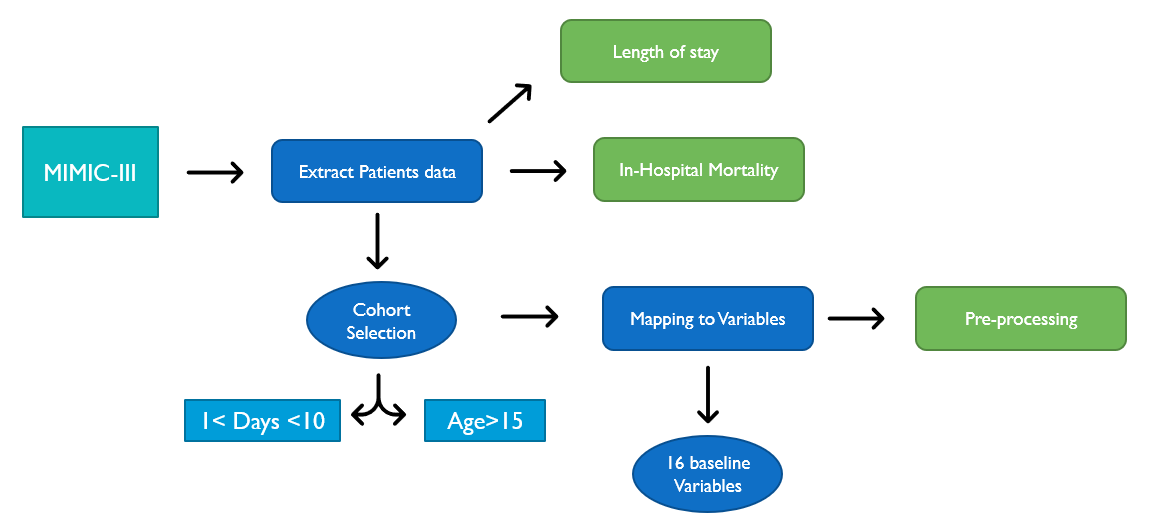
\includegraphics[width=\textwidth]{dissertation/Latex/images/Extraction pipeline.PNG}
\end{figure}



\subsection{Extracting patients data} 
    In this project, the tables admissions, icustays and patients is used to collect patients data that will be used to perform cohort selection on these patients. A inner join between patients data, admissions and icustays is performed to extract patients data including, gender, date of birth, date of death, admission time, dispatch time, deathtime, ethnicity and diagnosis information of all patients. 
    
    \textbf{Cohort selection} is an observational study often used in medical research to select groups of participants and followed a forward in time, to observe how likely a disease or an outcome is to develop within the group. In this project, cohort selection is used to observe the outcome of ICU-in hospital mortality within the patients. 
    
    The first selection requirement is for ICU admissions that \textbf{took at least a day and less than 10 days}. The first reason is to reduce the amount of imbalance data, for example, patients with a very short stay might not have sufficient recordings, and might affect the effectiveness of the imputation strategies applied in later stages. Another reason for selecting only ICU admission with less than 10 days is that if a patient is to stay in ICU for more than 10 days, there is a high possibility of being a special or extreme cases, which might result in irregular medical measurements. The second selection requirement is that the \textbf{admission patient must be of age >15}, since younger patients are still in development stage and their normal clinical indices might vary significantly compared to adults.
    
    After cohort selection, there are 30063 patients with 24 columns of data about these patients in the dataframe. The sql query used for extracting patients and cohort selection can be found in appendix \ref{appendix:patientsSQL}.


\subsection{Extracting Vital data and mapping to variables}

The next step to the extraction pipeline is to extract medical recordings for each patient from chartevents and labevents table mentioned earlier. Before doing so, we must first define the variables we would like to keep. For this project, we selected 16 variables as the baseline of the extraction pipeline, which includes: 

\begin{center}
   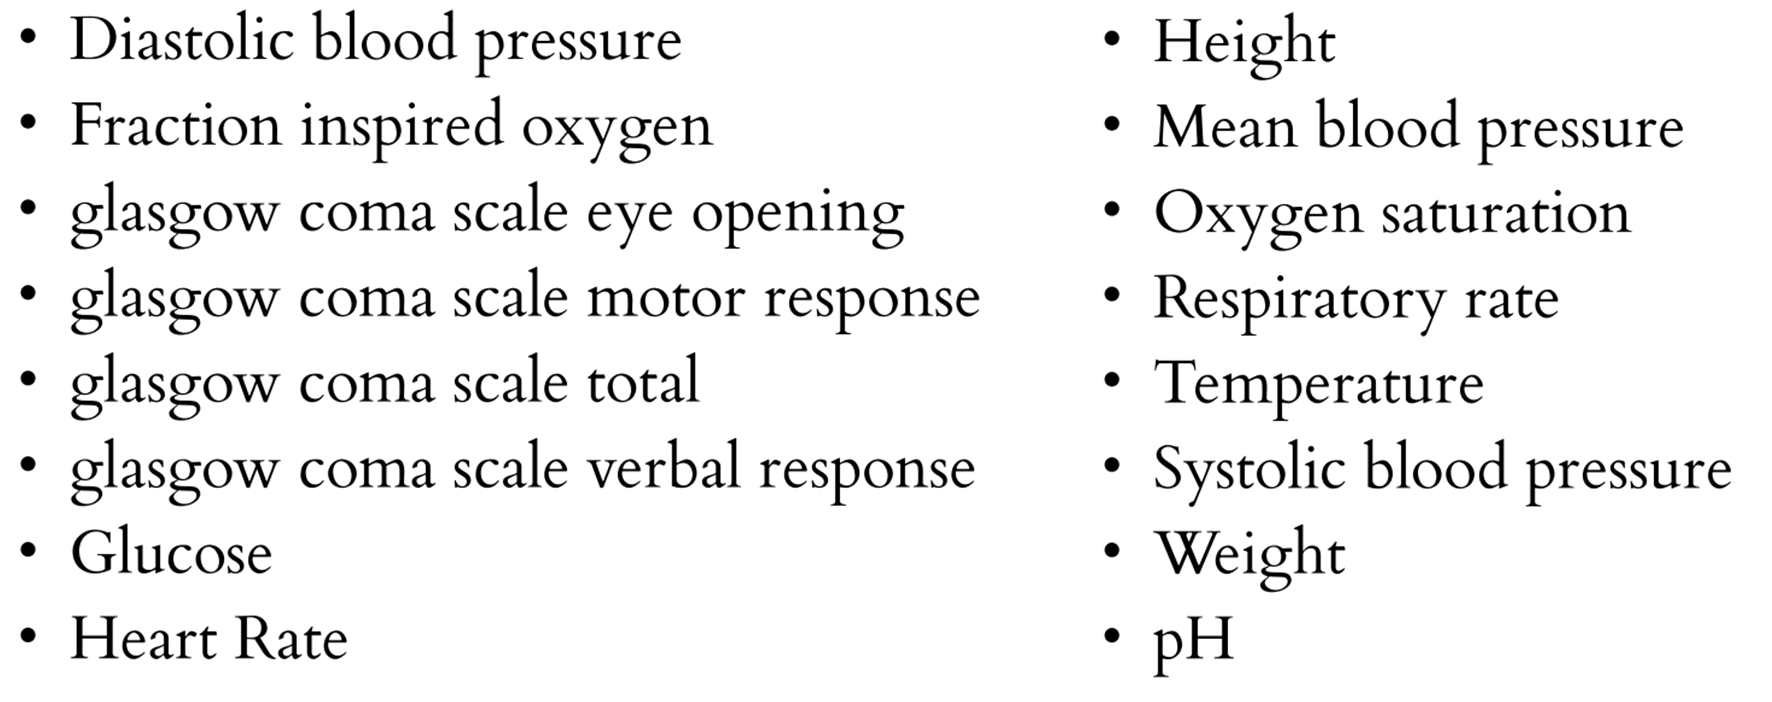
\includegraphics[width=8cm]{dissertation/Latex/images/baseline variables.PNG}
\end{center}


Using the itemid\verb|_|to\verb|_|variable\verb|_|map.csv resource file from \cite{MIMIC_Extract_Github}, we extract the itemid of these 16 variables and store them in a list of item id as variables to keep when extracting from events data. Using the list of icu id and hadms id from each patient along side the variables to keep list. The query used to extract events data can be found in appendix \ref{appendix:eventsSQL}.


At this stage, there is only itemid for each variable, and we do not know what item it is without it's label, we make use of the d\verb|_|items table from the dictionary table section of the database to map the label to the item id and also extract it's unit for unit conversions in later stage. 


\subsection{Extracting length of stay and in-hospital mortality}
Now that we have extracted all the information required for training our machine learning model, we also need to extract the clinical outcome of in-hospital mortality as labels for machine learning. It is also required to extract the length of stay in hours since we are only using patients that stayed for more than 48 hours. Both of these information can be simply extracted from the patients data we created in the first step.


\section{Formatting and Pre-processing Pipeline}


\begin{figure}[h!]
  \caption{Pre-processing Pipeline}
  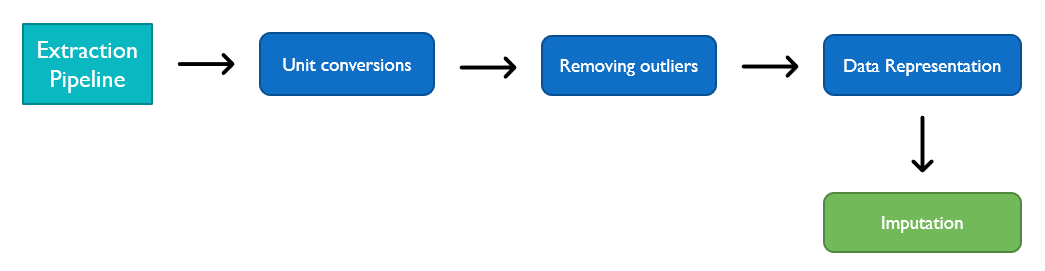
\includegraphics[width=\textwidth]{dissertation/Latex/images/Preprecessing pipeline.PNG}
\end{figure}


After all necessary data is extracted, we have to format and do some basic pre-processing before we could apply any imputation strategies and create the machine learning model. The 4 steps include unit conversion, removing outliers, data aggregation and finally reshaping the data.

\subsection{Unit Conversion}
Since different medical staff might measure the units differently, unit conversion is crucial in medical data since the meaning of the data could drastically change if not handled with care. Unit conversions are done manually by defining a list of tuples with the format of ('variable','unit','condition','conversion function'). An example for weight to conversion to kg would be ('weight','oz',  None,lambda x: x/16.*0.45359237) and ('weight','lbs', None, lambda x: x*0.45359237). The condition field is for variables like oxygen saturation where it is a percentage then the condition value is used to only apply the function when the value is larger than 1, and convert the percentage to a value between 0 to 1. ('oxygen saturation', None,  lambda x: x <= 1, lambda x: x*100.) This tuple is then used while looping through all the values within the events data and replace the value if inconsistent unit is found.


\subsection{Removing outliers}
For variables in medical data, there are often a range for possible values, and outside of that range, it is highly possible there was something wrong with the data collection process such as typing mistakes from the medical staff. A resource file from \cite{MIMIC_Extract_Github} called variable ranges is used as reference to decide whether the value in events data is within the variable range. The resource file contains 5 fields, outlier low, valid low, impute, valid high and outlier high. If the value of the variable is within the outlier low and outlier high value, this indicates the value is outside of the scientific range, thus will be treated as an outlier and replaced with a NAN value for later imputation. If the value is close to the valid low and high value, it indicates that the value is abnormal, but still within scientific range, therefore will not be replaced with the impute value. For example, Heart rate has a outlier and valid low of 0, impute value of 86, valid high of 350, and outlier high of 390. 

\subsection{Data Representation}
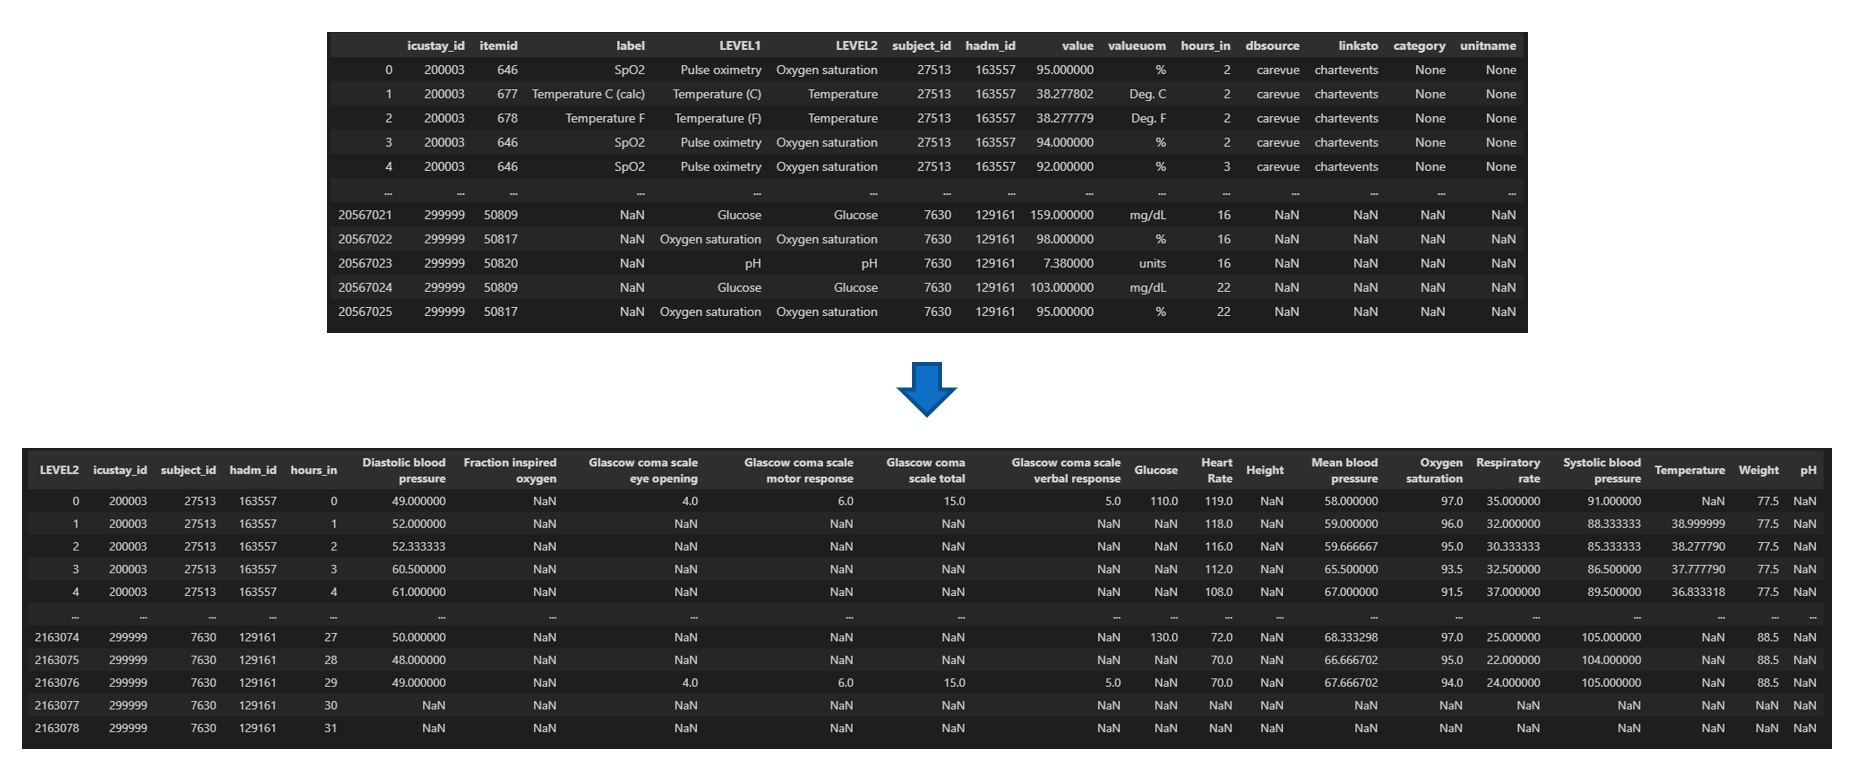
\includegraphics[width=\textwidth]{dissertation/Latex/images/reshape.PNG}

The final step is to simply reshape the original data with a row for every value to so that it has a column for every variable, and a row for every hour so that it is suitable for machine learning, where each column is treated as a feature. However, by reshaping data this way, it generates a lot of Nan values since there are obviously no recordings of every single variable once every hour. Since machine learning models cant learn with null values, this is where imputation comes in to fill in all these missing values. 

%==================================================================================================================================
\chapter{Implementation of Imputation Strategies}

After the extraction and formatting pipeline there are 843312 samples, which includes 17659 unique patients across 48 rows for each hour (17659*48=843312) and 16 variables for each row.The following is a snippet of the starting data frame for imputation:

\begin{figure}[h!]
  \caption{Non imputed data sample}
  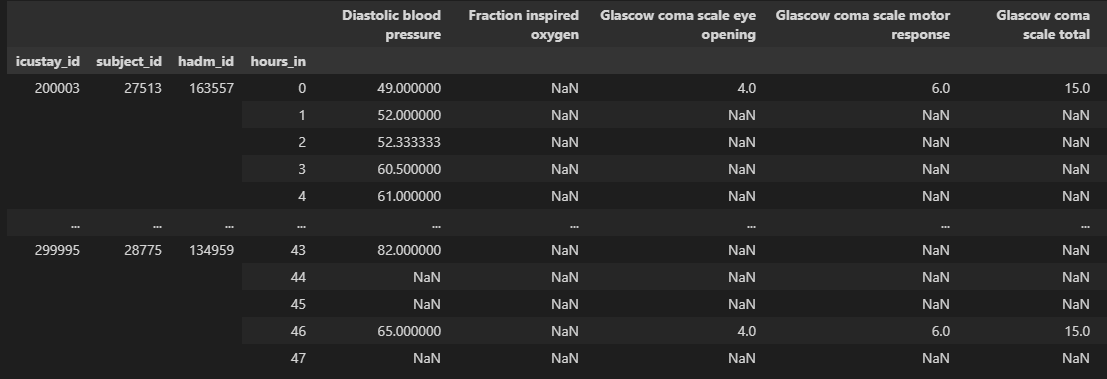
\includegraphics[width=\textwidth]{dissertation/Latex/images/Imputation Figures/non_imputed_data_sample.PNG}
\end{figure}


The imputation strategies used will be sectioned into two categories, \textbf{univariate} and \textbf{multivariate}.  

\section{Univariate imputation}


\begin{figure}[h!]
  \caption{Univariate Imputation}
  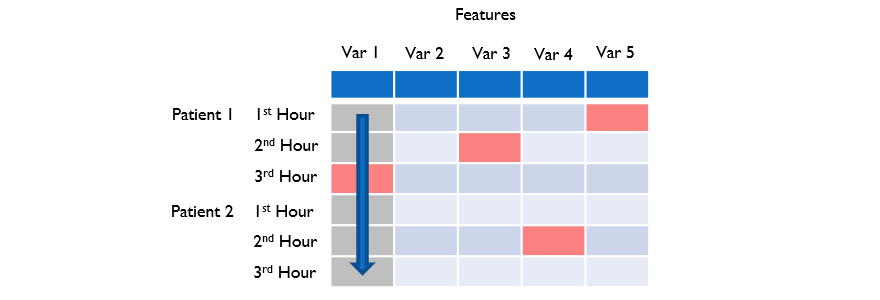
\includegraphics[width=\textwidth]{dissertation/Latex/images/Imputation Figures/univariate.PNG}
\end{figure}



The first type of imputation strategy is univariate, where the missing values within the feature is imputed only by non-missing values within the same feature of the same dimension (highlighted as gray in the diagram above). The univariate imputation strategies used are mean imputation and most-frequent imputation, which will both be implemented using the SImpleImputer class from SkLearn.


\subsection{Mean imputation}

\begin{figure}[h!]
  \caption{Mean imputation pipeline}
  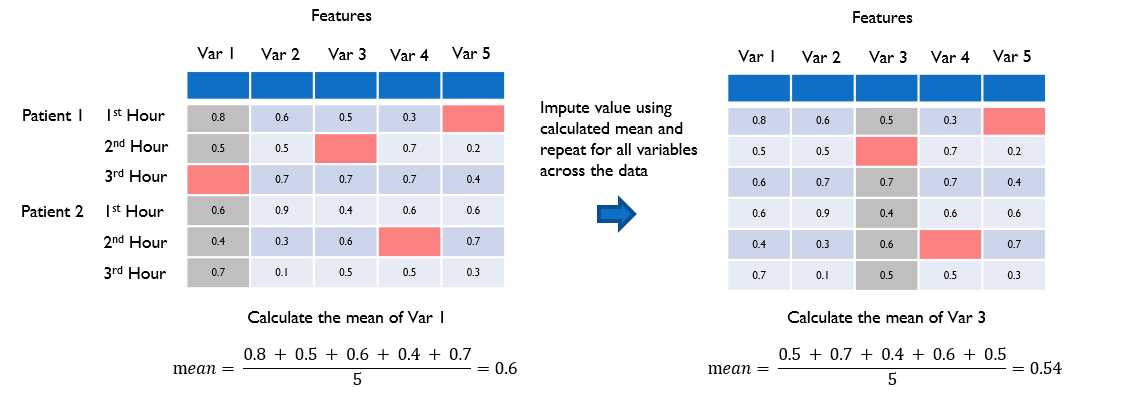
\includegraphics[width=\textwidth]{dissertation/Latex/images/Imputation Figures/mean imputation.PNG}
\end{figure}


Mean imputation is the method of filling missing values where the mean of the observed value is computed for each variable, and this mean is used to fill in all the missing value in this column. Figure 5.3 illustrates the mean imputation pipeline visually. Although mean imputation is easy to implement, it does not work well with categorical feature and often introduce bias to the dataset.



\subsection{Most frequent imputation}

\begin{figure}[h!]
  \caption{Most frequent imputation pipeline}
  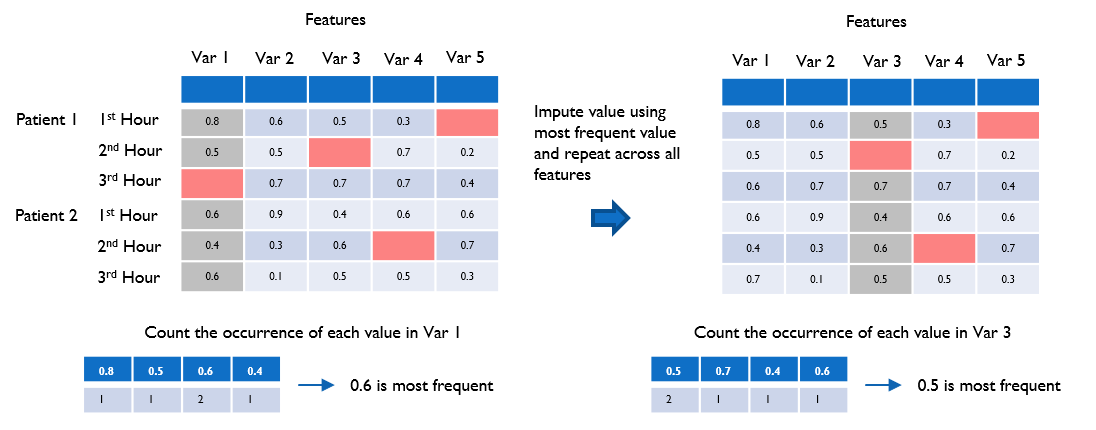
\includegraphics[width=\textwidth]{dissertation/Latex/images/Imputation Figures/most frequent.PNG}
\end{figure}


Most frequent imputation is the method of filling missing values using the most frequently seen value within each feature. This strategy is similar to mean imputation but since it is not taking the average of the values, it works better with categorical features. However similar to mean imputation, this method introduce bias to the imputed data. Figure 5.4 illustrates the most-frequent imputation pipeline visually.

\pagebreak

\section{Multivariate imputation}



\begin{figure}[h!]
  \caption{Multivariate Imputation}
  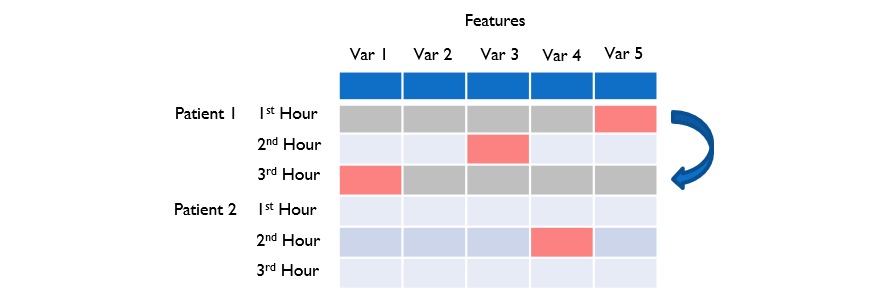
\includegraphics[width=\textwidth]{dissertation/Latex/images/Imputation Figures/multivariate.PNG}
\end{figure}


The second type of imputation strategy is multivariate, where when imputing a missing value, instead of only considering values from the same feature, these strategy consider the data in multi-dimension for all features and uses the full set of data to estimate the missing values.


\subsection{K-Nearest-Neighbor (KNN)}

K-Nearest-Neighbor (KNN) imputation is a distance based imputation method that utilizes the KNN algorithm, a non-parametric supervised learning method that could be used for both classification and regression. 

 \begin{figure}[h!]
  \caption{KNN imputation pipeline}
  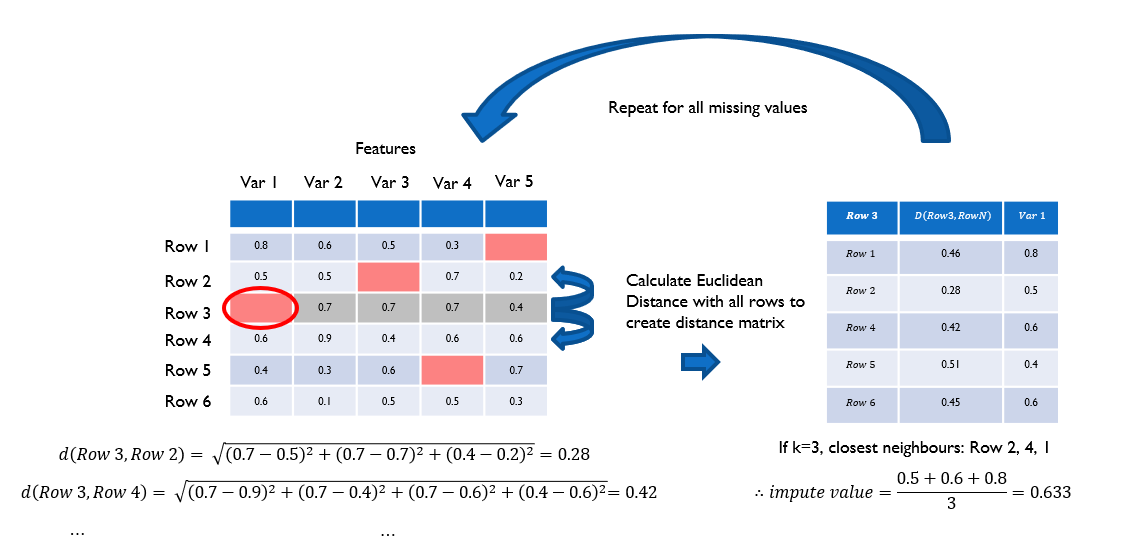
\includegraphics[width=\textwidth]{dissertation/Latex/images/Imputation Figures/KNN imputation.PNG}
\end{figure}

To use the KNN algorithm with imputation, we chooses it's closest neighbor by euclidean distance, which can be represented by the following equation in high dimensional space for each row combination {p} and {q} with element {i}:

 \[d\left( p,q\right)   = \sqrt {\sum _{i=1}^{n}  \left( q_{i}-p_{i}\right)^2 }\]
 
 Since missing values might be encountered when calculating the euclidean distance of each row, and NAN subtracted by anything is also NAN, that element pair will simply be ignored in the calculation. After all euclidean distance are calculated for all row combinations, the K rows with a non missing value in the same feature with of the lowest euclidean distance will be selected. The missing value is then replaced by the average value of its nearest neighbors for the same feature. This process is then repeated for all missing values. 
 
 Although calculating euclidean distance is not computationally demanding, since a distance array between all rows is calculated for each missing value, the KNN imputation method is extremely slow due to the nature of this algorithm, which took around 21 hours to impute the data we used above. 




\subsection{Multiple imputation by chained equations (MICE)}

Multiple imputation by chained equations (MICE) is a multivariate imputation strategy that imputes missing data through an iterative series of predictive models. Creating multiple imputations rather than single imputation takes considerations into the statistical instability and uncertainty in the imputations, while being flexible with both numerical and categorical variables.

 \begin{figure}[h!]
  \caption{MICE imputation pipeline}
  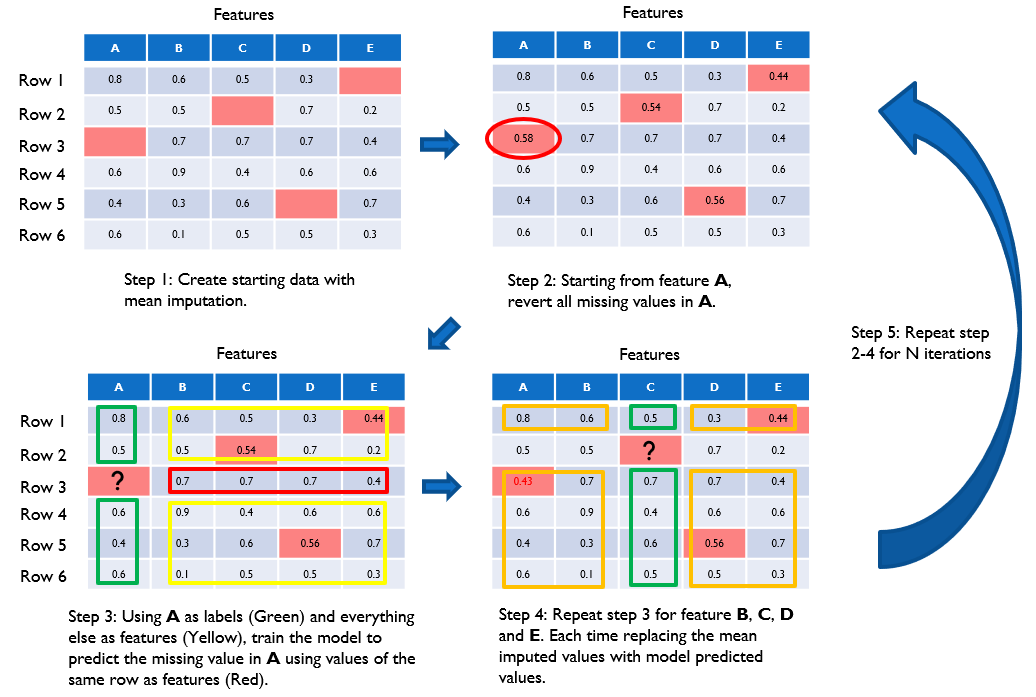
\includegraphics[width=\textwidth]{dissertation/Latex/images/Imputation Figures/MICE imputed.PNG}
\end{figure}

The MICE algorithm often start by using mean imputation or random predictions to fill up all the missing data, since we could not apply the predictive model if there are missing values in the data. For each iteration, the algorithm starts by selecting a feature and reverting it's missing values to null, which will later be filled by the predictive model we train. To obtain the train data for the model, the non missing values in the selected feature will be used as the true labels, and the other features in the same row will be used as the features for predicting that label. After training, we then predict the missing values giving it's other features of the same row as test data to obtain our first imputed feature. After replacing an entire column of mean imputed missing values with model predictions, we move on to the next column, reverting all it's missing values and apply the same steps to training and predicting the missing values. This process is then repeated across the whole data until there are no more mean imputed data but only model predicted data, which is where the first iteration ends. The same algorithm is then applied for multiple iterations until the imputed values converges, it often takes less than 5 iterations.

This algorithm is implemented with the MIMIC-III data using the MiceForest package, (\cite{wilson_2022}). It utilizes light gradient boositng machine (Lgbm) and has memory efficient capabilities to perform multiple imputation without copying the dataset. In this project, multiple customisation are made to fit the MIMIC-III dataset including performance boosting strategies like hyperparamter tuning. In order to further improve the statistical instability of imputation and remove uncertainty, we generated 4 different datasets using the MICE algorithm then compute the mean of these datasets. 



\subsection{Multiple Imputation with Denoising Autoencoders (MIDAS)}

Multiple Imputation with Denoising Autoencoders (MIDAS) is an imputation method recently proposed by \cite{lall_robinson_2022}. To begin with, autoencoders are a class of unsuperivsed neural network learning technique that leverage networks for the task of learning efficient codings for unlabled data. A denoising autoencoder is a subclass of an autoencoder that uses dimensionality reduction to preserve the key features of the signals while discarding noise. It learns to remove noise by corrupting the data on purpose to make the autoencoder more robust and to also learn more features compared to a standard autoencoder. The denoising autoencoder corrupts a subset of the input data by injecting stochastic noise, then attempt to recontruct these corrupted data through a series of nested nonlinear transformations. The MIDAS imputation approach re-purposed denoising autoencoders by treating missing values as an additional portion of the corrupted data at the beggining stages of denoising autoencoders, and paired this with multiple imputation with the aim to capture more complex relationship between different variables and more accurate imputation.


 \begin{figure}[h!]
  \caption{MIDAS imputation pipeline}
  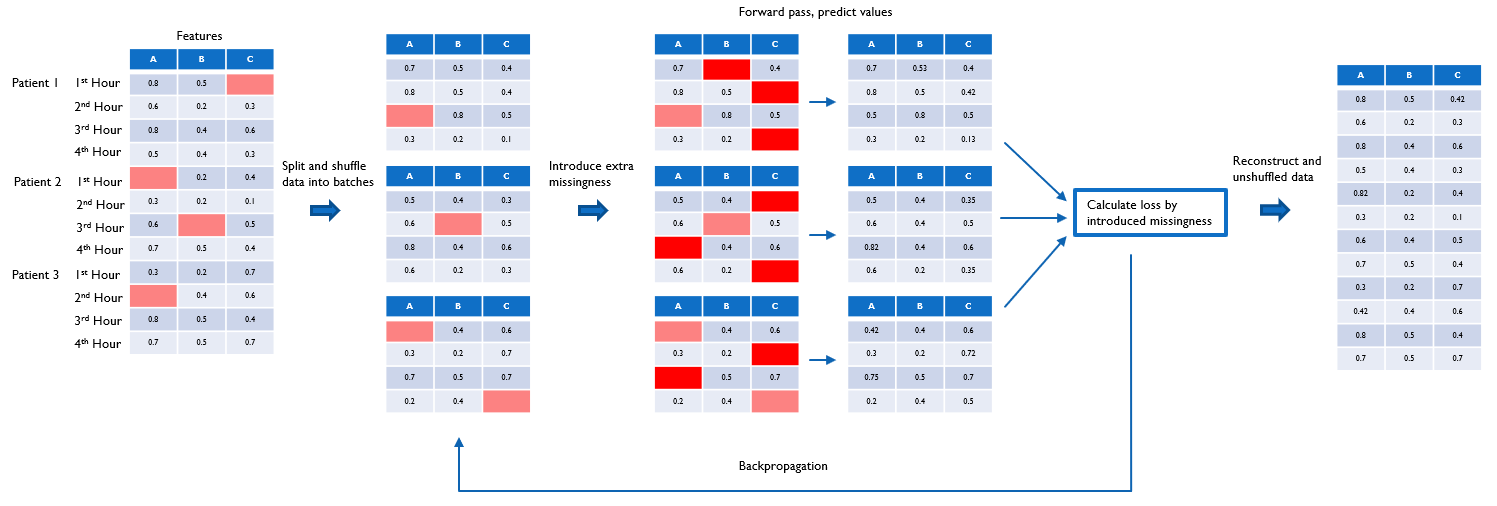
\includegraphics[width=\textwidth]{dissertation/Latex/images/Imputation Figures/MIDAS imputation.PNG}
\end{figure}

The training of the MIDAS algorithm consist of five main steps which is summarised in figure 5.8, the algorithm first shuffle and slice row-wise data in paired mini-batches, this is done to accelerate the converge rate of the model, \cite{lall_robinson_2022}. The second step partially corrupts these these mini batches through multiplication by a bernoulli vector to introduce noise. This third step applies a standard implementation of dropout, a regularisation technique used to reduce over-fitting by introducing more missing values to the neural network. The fourth step involves a forward pass through the denoising auto-encoder, which predicts a value for all the missing values,the loss is then calculated using the loss function. The fifth step aggregates the loss values into a single term and backpropagates through the denoising auto-encoder, with the resulting error gradients used to adjust the weight for the next iteration. For a more detailed explanation of MIDAS, checkout the original paper for MIDAS by \cite{lall_robinson_2022}.

\section{Leave one out cross validation (LOOCV)}

For evaluating how closely the imputed data resembles the original data, a Leave one out cross validation (LOOCV) procedure inspired from the paper \cite{Nijman2021} is used. The process involves selecting a random data point for each patient across all columns, replacing it with an empty value, then comparing the predicted value from the imputation algorithm for each datapoint. The same procedure is then repeated multiple times with another random set of selected data points for each patient, this cross validation step is to prevent over-fitting and making assumptions with only one test. 

The predicted value by the imputation algorithm is then collected compared to it's original true value by using root mean squared error along side the coverage rate and average width.

 
 
\section{Clinical Decision Prediction Model}
After applying all the imputation strategies on the starting data-frame, the imputed datasets are preprocessed then used to train machine learning models separately using cross validation to predict in-hospital mortality of the patients.

\subsection{Removing outliers }
Since it is possible that outliers are introduced again during the imputation process, the process used during the extraction pipeline to remove outliers is repeated for the imputed dataset using the variable ranges.

\subsection{Minmax scaling}

Since variables within the model is measured using different units and do not contribute to the machine learning model equally, min max normalisation is applied to the data to prevent bias. It can be represented by equation 5.1, where \({x}_i\) is the current value, \(x_\text{min}\) is the min value in the row, and \(x_\text{max}\) is the max value in the row.

\begin{equation} \label{eq:1}
\tilde{x}_i=\frac{x_i - x_\text{min}}{x_\text{max} - x_\text{min}}
\end{equation}


\subsection{Undersample majority}

As mentioned earlier, the mortality rate of the starting dataset is around 13 percent, meaning that more than 80 percent of the data is identified as the same class within the training data. With such extreme cases of imbalance data, there is a high chance that the model with overfit to the majority class and create biased prediction. To prevent this, the under sample majority function is used to undersample the data by selecting the same number of data from the class with the fewest data, so that the number of training data for each class is the same. Using this approach means introduces major disadvantages as we are neglecting alot of data. However, if the problem of class imbalance is not solved, the model will make biased predictions of one class only, which is even worse.

\subsection{K-Fold cross validation}

K fold cross validation is a resampling method that splits the data into multiple train-test sets instead of the traditional trian test split. Within each split, the machine learning is trained and evaluated using it's train-tests sets, the results from each split are then accumulated and compared using different metrics.  This sampling method is used to ensure every observation from the datset is exposed to both training and test set in one of the splits. Since all values from the dataset is used in both training and testings, it allow fair testing for our imputed dataset and comparison of effectiveness of these trained models with least amount of bias.



%==================================================================================================================================
\chapter{Results and Evaluation} 

\section{Missingness of data}
The first step to the evaluation pipeline is to evaluate the missingness of our data before imputation. Figure 6.1 and 6.2 shows the number non missing data for each variable within the dataframe out of the 8343312 rows using a barplot and matrix plot respectively. 

\begin{figure}[!htb]
  \caption{Bar plot of data before imputation}
  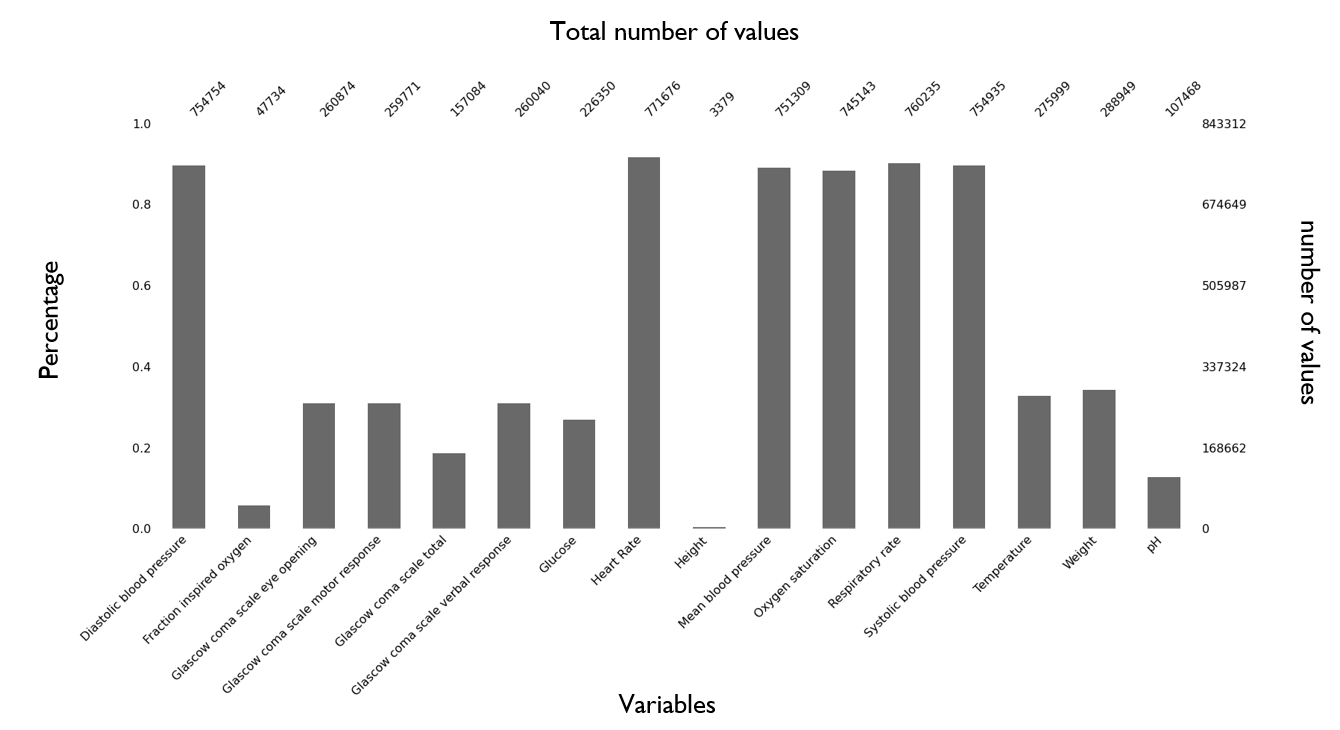
\includegraphics[width=\textwidth]{dissertation/Latex/images/Missingness Figures/barplot.png}
\end{figure}

\begin{figure}[!htb]
  \caption{Matrix plot of data before imputation}
  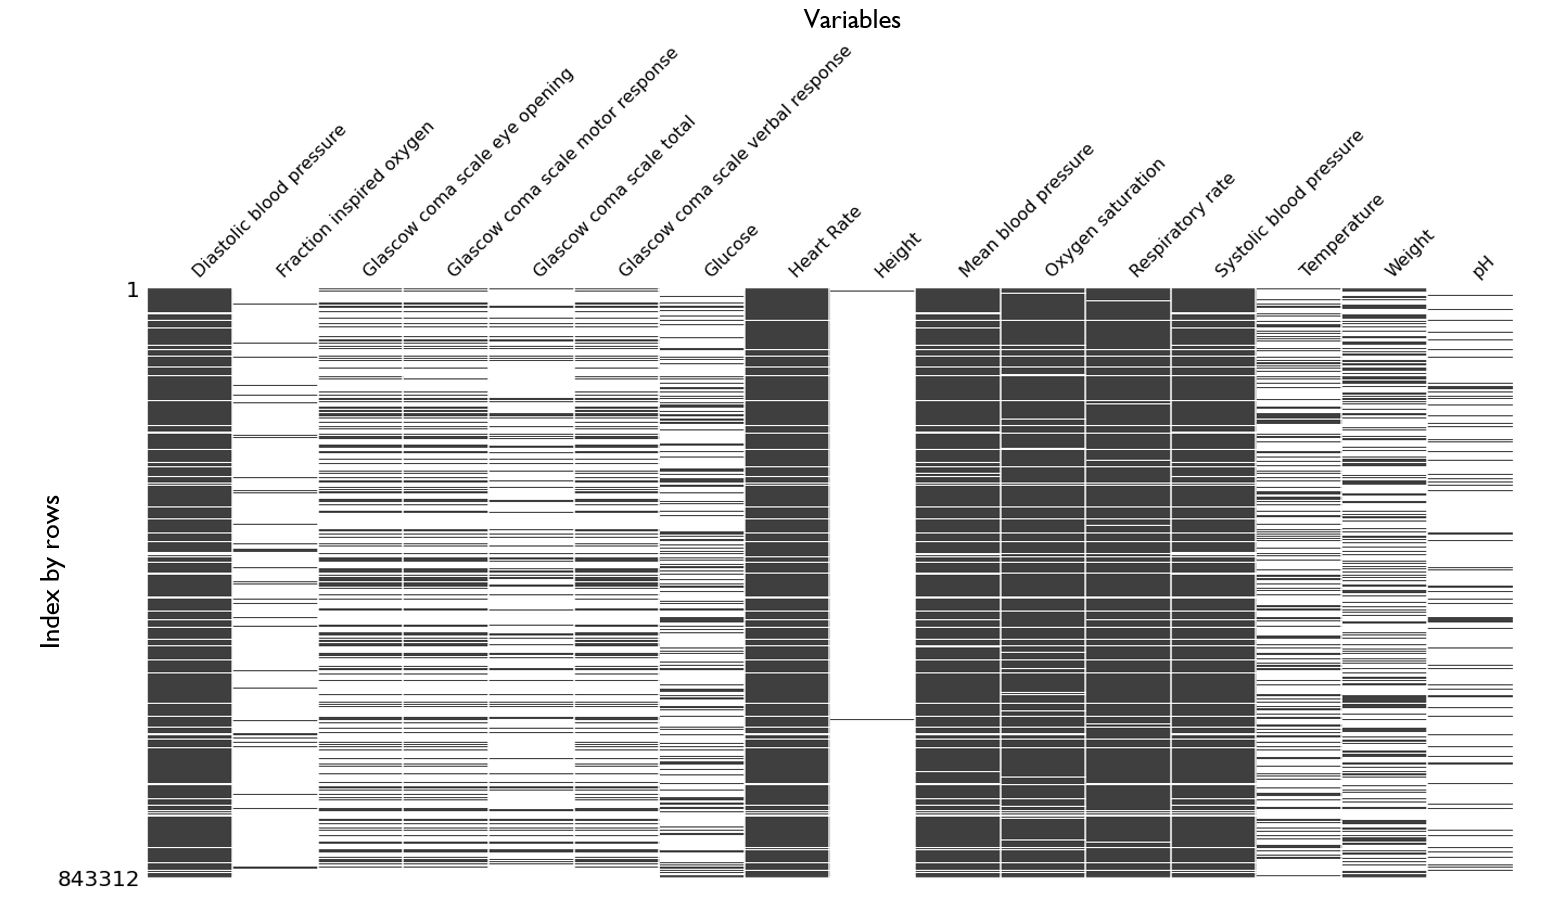
\includegraphics[width=\textwidth]{dissertation/Latex/images/Missingness Figures/matrixplot.png}
\end{figure}

We see from the bar chart in figure 6.1 that Diastolic blood pressure, heart rate, mean blood pressure, oxygen saturation, respiratory rate and systolic blood pressure are the only 6 variables with more than 80 percent of it's data present within the dataframe. One thing these 6 variables have in common is that these common medical measurements are that are regularly measured and monitored for all types of ICU patients. We could observe in the matrix plot from figure 6.2 that the missing data for these 6 variables are widely spread randomly across the data frame, suggesting that the data missing mechanism is at random (MAR). This missing at random might be due to various reasons including the moving of patient within the ICU unit or a medical staff forgetting to take the recording etc. 

From figure 6.1, we also see that fraction inspired oxygen and height has the least recordings with less than 10\% of its data present. Looking at the figure 6.2 for these two variables, we see that height is very rarely measured by the medical staffs. The reason behind this might be because patients in the ICU units are often in severe medical conditions, which makes measuring their height difficult. Observing where the missing values are located for fraction inspired oxygen, we see that there are lots of wide gaps between recordings, suggesting only some specific patients require this test and it is not a variable as common as more standard variables like heart rate and diastolic blood pressure. This suggests that there are information hidden behind these missingvalues and are examples of variables missing not at random (MNAR), since there are obvious reasons to why these recordings are taken less often than other ones.

For other variables, they are mostly around the 20\% to 40\% range for number of values present within the dataframe, we see that for glasgow coma scale eye opening, motor response, and verbal response, the number of values and location of these values is exactly the same from figure 6.1 and 6.2, showing the recordings are taken along side each other for patient. This is highly possibly due to this score only used for patients with impaired consciousness, suggesting these values are MNAR. However for temperature and weight, we see from 6.2 that the values are spread relatively randomly, suggesting it is MAR.

By analysing the missingness of the data, we see that unlike traditional data where there is only one type of missingness, each medical variable within the data has different type of missingess and we can deduce logically the reasoning behind such missingness. This suggests that it might be useful to identify what type of missingness each medical variable has, then apply specific imputation strategies accordingly for the best results. Some imputation strategy might be more effective for a certain type of missing data, so this could be an interesting subject in future researches.

\section{Qualitative comparison of Imputation methods}



\begin{figure}[!htb]
  \caption{Comparison of probability distribution curves for diastolic blood pressure}
  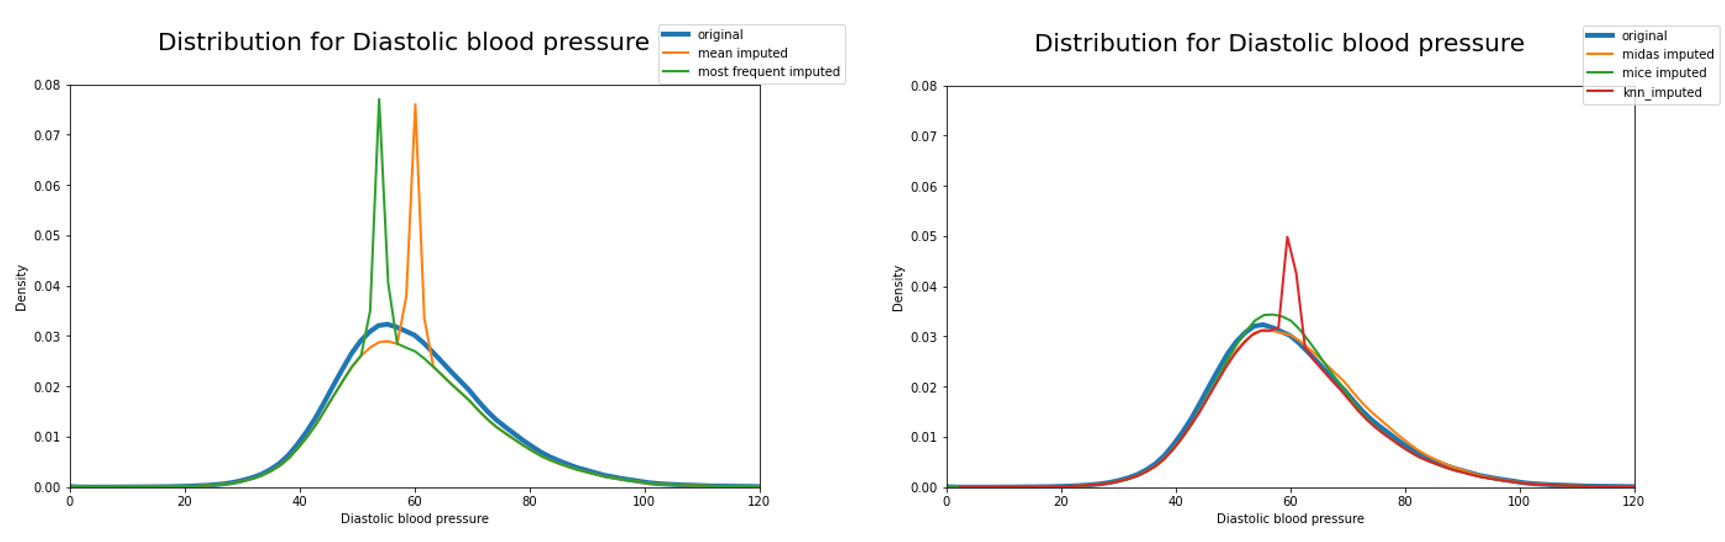
\includegraphics[width=\textwidth]{dissertation/Latex/images/Diastolic blood pressure distribution.PNG}
\end{figure}


By plotting the distribution of the original data and imputed data, we could visualise how similar the imputed data is to the original data. For better visualisations and analysis, glucose and blood pressure is selected as examples, uni-variate and multi-variate imputation strategies is separated into two graphs. The full distribution can be found in appendix \ref{appendix:distributions}.

Looking at the MIDAS imputed and MICE imputed curves on the right of figure 6.3, it resembles a smooth Gaussian distribution similar to the original curve. On the other hand for KNN imputed, mean imputed, and most frequent imputed data, we see huge spikes for certain values. These huge spikes in the distribution is suspected to be caused by nature of these algorithms. For mean imputation, the same value for the each column is replicated throughout the entire column, and for most frequent it replicates the closest non-missing value. As for KNN imputation, despite being a multivariate imputation method, the algorithm still takes the mean of it's value in the same column after finding it's nearest neighbors in terms of the entire row, therefore replicating a similar but smaller spike the same with mean imputation. However, if we look at the missingness of Diastolic blood pressure, only around 10 percent of data is missing for this variable, lets look at another example that has more missing values.

\begin{figure}[!htb]
  \caption{Comparison of probability distribution curves for glucose}
  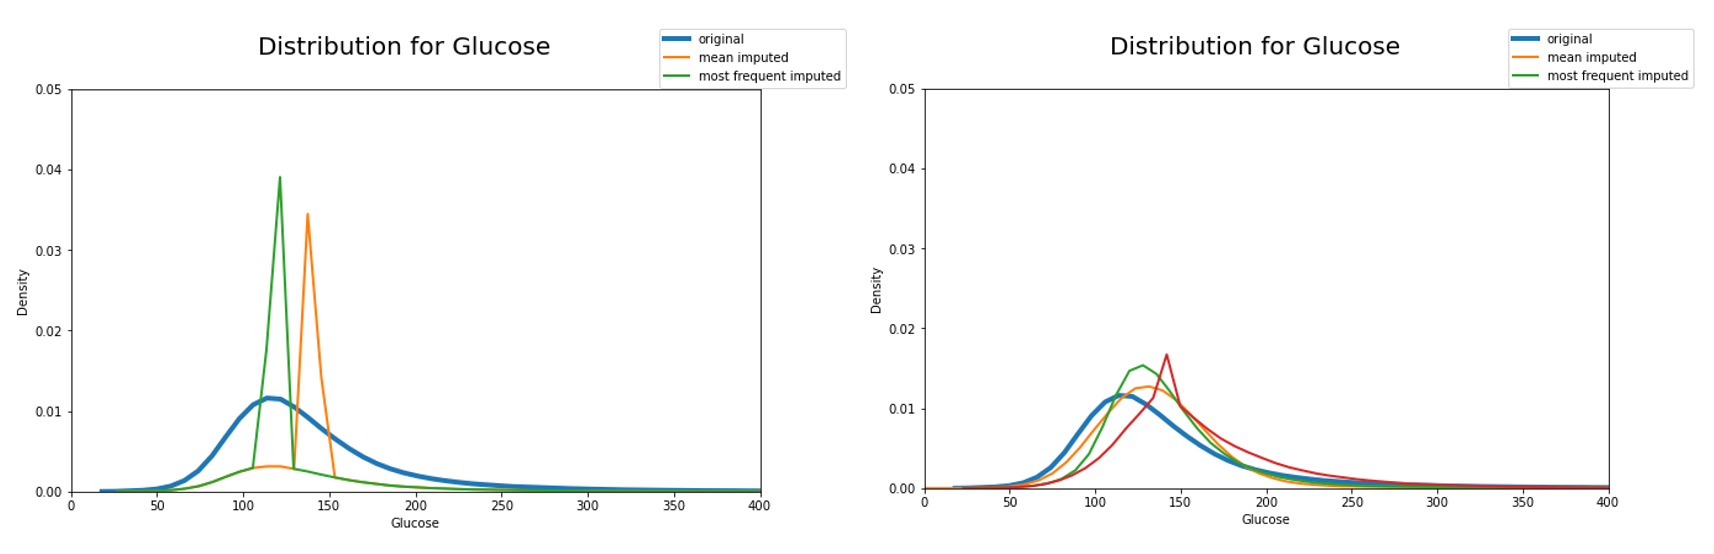
\includegraphics[width=\textwidth]{dissertation/Latex/images/Glucose Distribution.PNG}
\end{figure}


Looking at the distribution graphs for glucose, we still see a near identical spike pattern for mean imputation and most frequent imputation. As for the multivariate imputed data, the curve is less similar to the original data due to the fewer samples available for the machine learning algorithms to learn and perform more accurate predictions. As for the KNN imputed data we observed a similar spike and the curve is also less smooth compared to the other algorithms.The problem with the spikes could possibly be fixed with a higher number of k neighbors, but due to the slow nature of the algorithm and the large data set, hyper-parameter tuning and optimizing the KNN imputation method is not too realistic with limited resources.

From analysing the distribution graphs, we could hypothesis that multivariate imputation methods are capable of imputing results more similar to the original value compared to univariate imputation strategies even with fewer data to start with. To further prove this hypothesis, we could evaluate the RMSE in the holdout value simulation in the next section.

\pagebreak


\section{Quantitative Evaluation based on Simulation Data}

The leave one out cross validation method is used as a holdout experiment for our imputation strategy. To conduct this experiment, the imputation process is repeated multiple times separately with extra missingness introduced to the data, so it would also affect the effectiveness of univariate imputation strategy disadvantageously. However, this effect is minimal and this experiment is crucial to identify how effective the imputation strategies are to recreate the original data.

Another important note of literature is that imputation is not prediction, where this idea was first introduced in an early paper by \cite{Gleason1975}. A more recent book from \cite{buuren_2021} described this issue that being successful in a simulation with both true and imputed value could not entirely represent the effectiveness of the imputation. This is because in imputation, the values we replace are missing values that has inherit uncertainty, meaning these values are missing after all and we cannot just assume as if it was not missing originally. This also means that more advanced imputation more capable of creating values more similar to the original might introduce bias and ignore the inherit uncertainty of this data. Therefore, the aim of this LOOCV simulation is not to evaluate how successful the imputation strategy is, but only to evaluate how capable each impuation strategy is to impute values that closely resembles the original.

\subsection{Root mean squared Error}
To measure the similarity between the imputed and original holdout values, the metric root mean squared error (RMSE) is used. This measure penalizes the larger error and is more sensitive to extreme values. Mathematically, it is a compromise between bias and variance, which evaluates the predicted value on both accuracy and precision. To minimize the bias in this simulation, the standard deviation for each fold of our cross validation is represented by the error bars in figure 6.3 so that we could see how the mean squared error varied for each iteration. RMSE can be represented by equation 6.1, Where \(n_\text{miss}\) is the number of missing values,  \(y^{true}\) is the true value, and \(y_i^{pred}\) is the predicted value by imputation.

\begin{equation} \label{eq:1}
RMSE = \sqrt{\sum_{i=1}^{n_\text{miss}}(y_i^{true}-y_i^{pred})}
\end{equation}


\begin{figure}[!htb]
  \caption{mean RMSE comparison for LOOCV}
  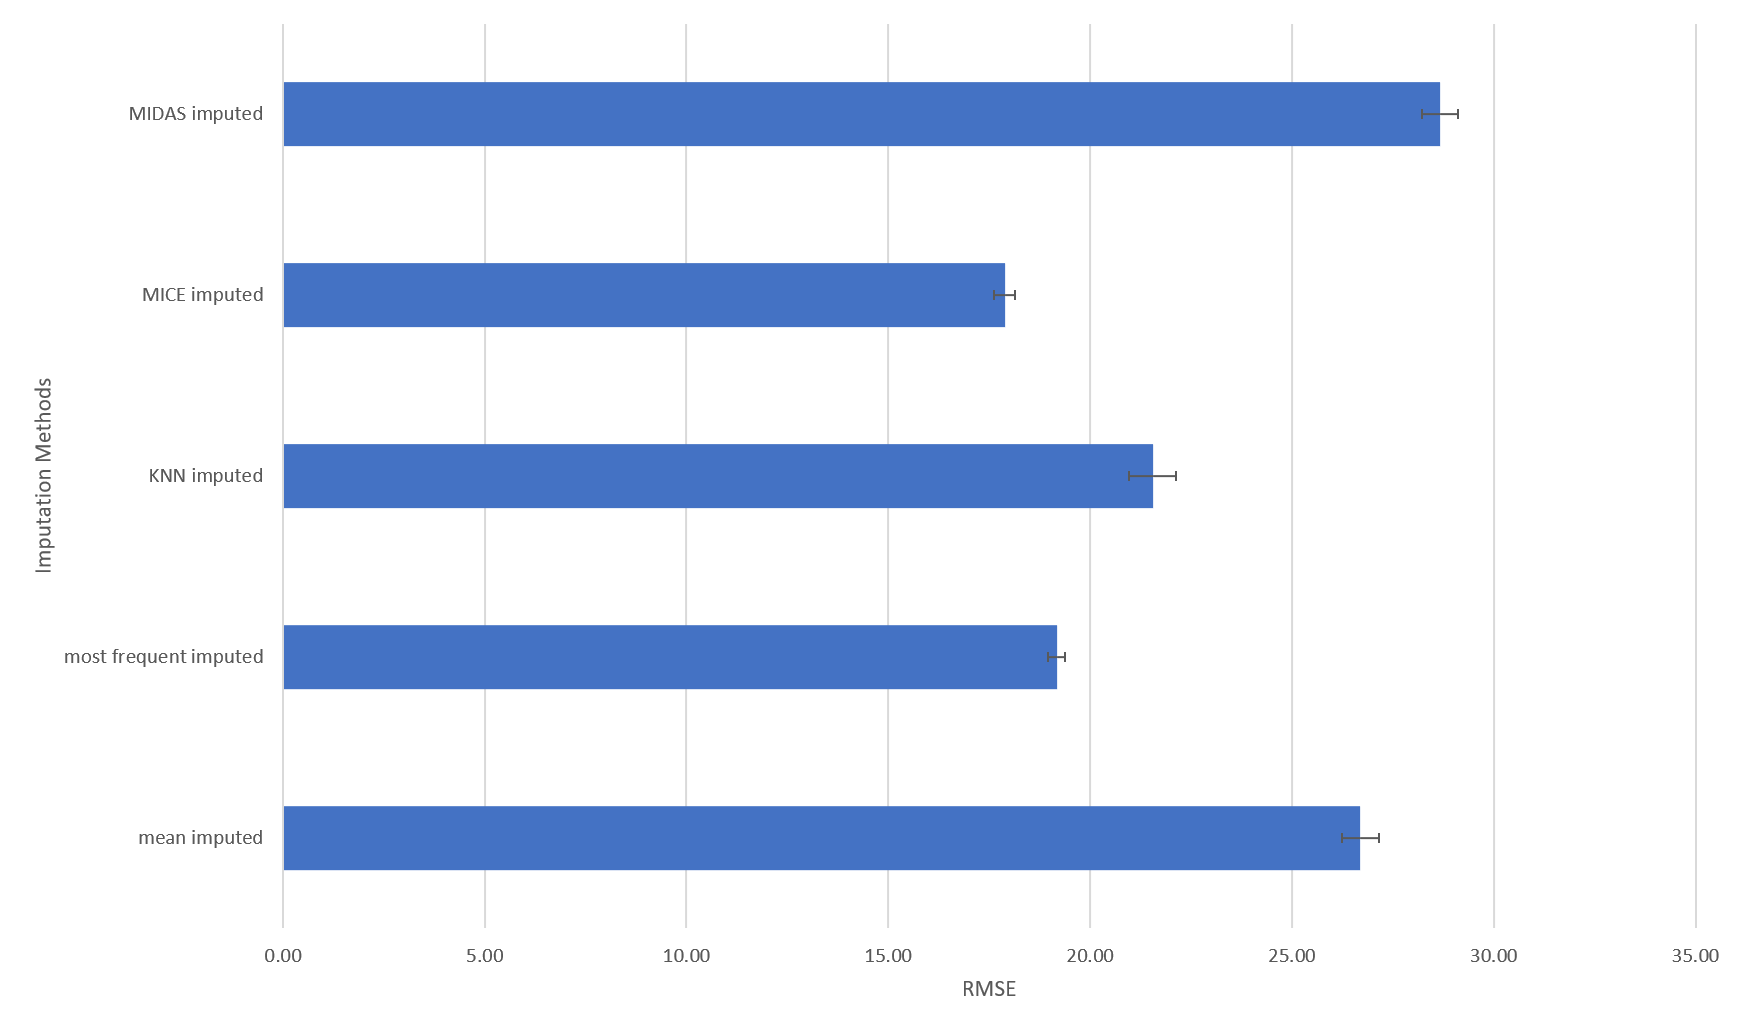
\includegraphics[width=\textwidth]{dissertation/Latex/images/holdout_rmse.PNG}
\end{figure}


From looking at the summary bar chart in figure 6.3, we see that the MICE algorithm has both the lowest RMSE and lowest average RMSE across the 3 cross validation folds. We observed that the difference and uncertainty range for KNN and MICE is comparably lower than mean and most-frequent imputation. This is possibly due to huge spikes in the distribution in the previous section. Since the same value is repeated across the whole column, the average distance for each variable is bound to be quite high and also varies quite randomly by which data-point is selected.

Interestingly, we see that the deep learning approach has the highest RMSE, but this might not necessarily mean it is bad as an imputation strategy. From the book mentioned earlier by \cite{buuren_2021}, it said that measures based on similarity between true and imputed values do not separate valid from invalid imputation methods. This means that having a low RMSE suggest the potential of creating biased data during imputation, and high RMSE has less potential of creating over-fitted data that is more realistic. 

With evidence from the distribution graphs in section 6.2 and RMSE evaluation in the LOOCV experiment, we can conclude that the MICE imputation method has the best ability to impute data that closely resembles the original data both by distribution and RMSE from the holdout value experiment. On the other hand, MIDAS imputed data has the highest RMSE despite having similar distributions with the original data. To further evaluate the effectiveness of these imputation strategy, we could use these data to train a clinical decision model to predict in-hospital mortality in the next section.


\section{Performance Evaluation of Risk Prediction Models}
For further evaluation of effectiveness for each imputation strategy, the imputed data for each strategy is used to create a machine learning model separately with cross validation to predict in-hospital mortality. In-hospital mortality is a binary classification task, where 0 means the patient is alive after 48 hours and 1 means the patient is deceased. 3 different machine learning classifiers are used to perform this experiment: Logistic regression, Random Forest, and Support Vector Machine Classifier. 

\subsection{Performance Metrics}

For measuring the performance of the classification models, four metrics are used: f1-score
macro, accuracy, precision, recall. The confusion matrix and ROC curve will also be used to
better visualise the performance of the model.

\textbf{Accuracy} is the most fundamental metric to measure model performance, it measures the
number of correctly predicted outcomes over all the outcomes predicted.

\begin{equation} \label{eq:1}
Accuracy = \frac{True Positives + True Negative}{True Positive + False positive + True Negative + False Negative}
\end{equation}

\textbf{Precision} measures the proportion of predicted positives that are correctly classified. Therefore,
it is the number of true positives divided by the number of labels predicted positive.

\begin{equation} \label{eq:2}
Precision = \frac{True Positives}{True Positive + False positive}
\end{equation}

\pagebreak

\textbf{Recall} measures the proportion of actual positives that are correctly classified. Hence, it is the
number of true positives divided by the number of all truly positive labels.

\begin{equation} \label{eq:3}
Recall = \frac{True Positives}{True Positive + False negative}
\end{equation}

\textbf{F1 score} is the harmonic mean of precision and recall.

\begin{equation} \label{eq:4}
F1= 2 \times \frac{precision \times recall}{precision + recall}
\end{equation}

\begin{figure}[!htb]
  \caption{Logistic Regression 10 Fold Cross Validation summary}
  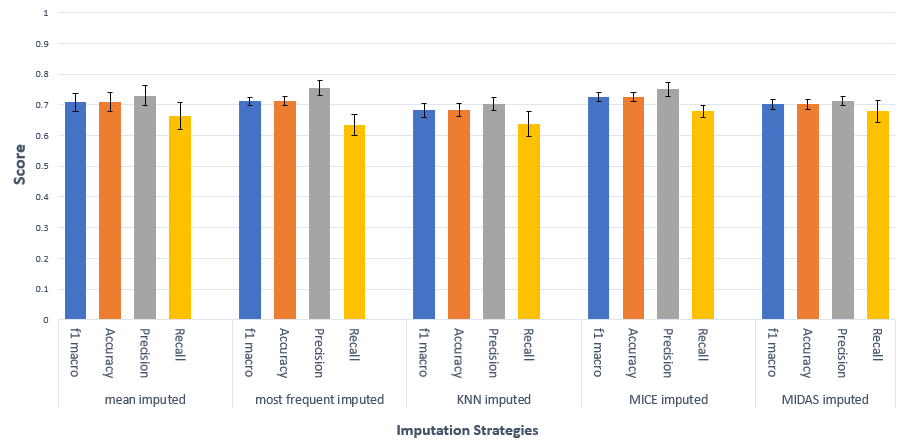
\includegraphics[width=\textwidth]{dissertation/Latex/images/Classification Results/lg_metrics.PNG}
\end{figure}

\begin{figure}[!htb]
  \caption{Random Forest 10 Fold Cross Validation summary}
  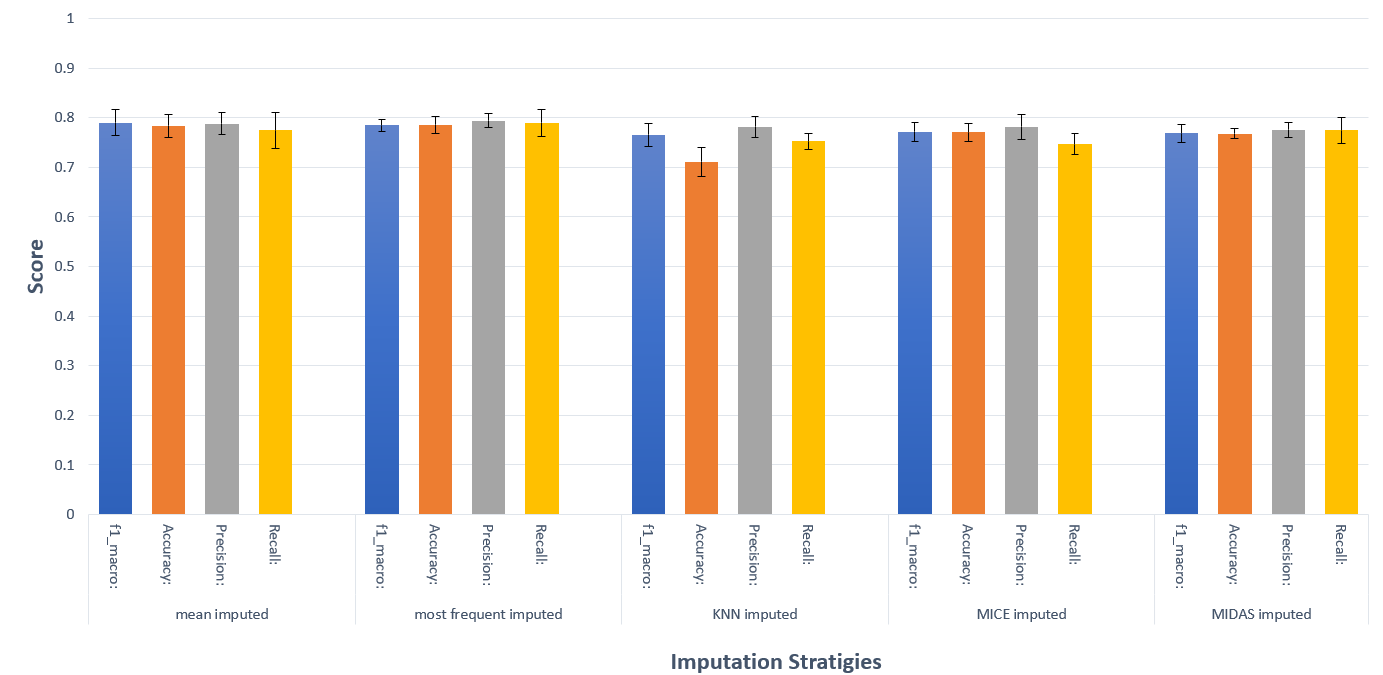
\includegraphics[width=\textwidth]{dissertation/Latex/images/Classification Results/10cv_rf.PNG}
\end{figure}
 
\begin{table}[!htb]
\centering
\caption{Logistic Regression 10 Fold Cross Validation Results}
\resizebox{\textwidth}{!}{\begin{tabular}{lSSSSS}
 Metric    & mean              & most frequent     & KNN imputed       & MICE imputed      & MIDAS imputed     \\ \midrule
f1 macro  & 0.708 (+/- 0.03)  & 0.711 (+/- 0.014) & 0.682 (+/- 0.022) & \textcolor{red}{0.725 (+/- 0.015)} & 0.701 (+/- 0.016) \\
Accuracy  & 0.709 (+/- 0.03)  & 0.713 (+/- 0.014) & 0.683 +/- 0.021)  & \textcolor{red}{0.726 (+/- 0.015)} & 0.702 (+/- 0.016) \\
Precision & 0.73 (+/- 0.034)  & \textcolor{red}{0.754 (+/- 0.025)} & 0.702 (+/- 0.021) & 0.75 (+/- 0.022)  & 0.712 (+/- 0.014) \\
Recall    & 0.663 (+/- 0.043) & 0.635 (+/- 0.034) & 0.636 (+/- 0.041) & \textcolor{red}{0.678 (+/- 0.02)}  & \textcolor{red}{0.678 (+/- 0.037)}  \\ \bottomrule

\end{tabular}}
\end{table}

\begin{table}[!htb]
\centering
\caption{Random Forest 10 Fold Cross Validation Results}
\resizebox{\textwidth}{!}{\begin{tabular}{lSSSSS}
Metric    & Mean              & Most frequent     & KNN imputed       & MICE imputed      & MIDAS imputed     \\ \midrule
f1 macro  & \textcolor{red}{0.790 (+/- 0.026)} & 0.785 (+/- 0.012) & 0.766 (+/- 0.023) & 0.772 (+/- 0.019) & 0.769 (+/- 0.018) \\ 
Accuracy  & 0.784 (+/- 0.023) & \textcolor{red}{0.786 (+/- 0.017)} & 0.771 (+/- 0.029) & 0.771 (+/- 0.018) & 0.768 (+/- 0.010) \\
Precision & 0.788 (+/- 0.022) & \textcolor{red}{0.794 (+/- 0.014)} & 0.782 (+/- 0.021) & 0.782 (+/- 0.025) & 0.776 (+/- 0.015) \\
Recall    & 0.775 (+/- 0.036) & \textcolor{red}{0.790 (+/- 0.027)} & 0.753 (+/- 0.016) & 0.747 (+/- 0.021) & 0.775 (+/- 0.026) \\ \bottomrule

\end{tabular}}
\end{table}

Figure 6.1 and 6.2 shows the logistic regression performance for all imputation strategies. Despite having similar performance if we look at the bar chart, We see that MICE algorithm performed the best with an mean f1 score of 0.725 across 10 fold cross validation. This is inline with existing literature that MICE imputation is a better imputation strategy all rounded. However for deep learning and knn imputation, we see that the performance of machine learning model using these imputed data performed consistently worse than mean and most-frequent imputed. We also see that the mean and KNN algorithm has a large uncertainty range, meaning the model trained using these imputed data are less stable and creates more diversed prediction. 

The fact that the mean imputation performed better than knn and deep learning imputed raises an interesting hypothesis that imputed data more similar to the original data does not necessarily mean this data creates a better performing machine learning model. If we compare KNN, mean, and most frequent imputed data by looking back at figure 6.5, we see that the mean imputed datset has higher RMSE in the holdout experiment than the KNN imputed dataset, while the most frequent imputed dataset had a lower RMSE compared to the KNN imputed dataset. However, despite the RMSE score of KNN being in between the two other methods, it had a consistently worse performing trained model. This shows that if the purpose of the task was only to create a more accurate machine learning model, mean and most frequent imputation should be chosen over the KNN and MIDAS imputation despite it being more capable to impute values more similar to the original data.

Looking at the results for random forest in 6.2, we see that it performs better in general compared to the logistic regression classifier, where mean imputation and most frequent imputation out performed our other models. However, one important thing we must consider is the disadvantages of single imputation techniques like mean imputation and most frequent imputation, despite the higher performance achieved by using these methods for random forest, these methods are often introduce alot of bias to our model and greatly reduce variance of the data set. We could see this by comparing the variance of the dataset in table 6.3, we see that the variance of mean and most frequnt imputation is significantly lower than the other 3 methods. 

Another important consideration is that despite efforts in using cross validation to minimize bias, the training and testing data is from the same dataset. Meaning if our imputed dataset is biased, not only the model trained is biased, but the testing is also biased. To solve this problem and create an unbiased testing environment, the only obvious solution is to have more natural test data from the medical dataset without any missing values in any columns, which is very few in the MIMCI-III dataset and not close to enough for a fair percentage split between train, validation and test. This describes a natural challenge when creating clinical decision models. It is unrealistic to have real life measurements for all the medical variables for every single hour, and it is hard to gather data without missing values for creating an unbiased model in clinical database environment.

\subsection{Hypothesis Testing}

Since the performances of our model is relatively similar for some classifiers, hypothesis testing is useful to determine if the difference in predictions our model made for each imputation strategy is statistically significant. The classification results for each of 10 folds is organised into an array for each imputation strategy. This is then evaluated using the friedman test to test the null hypothesis of if the f1-scores for each imputation strategy is equal. The alternative hypothesis is that at least one f1-score within the 10 folds is different for any of the imputation strategies. If the p-value of the friedman test is less than 0.05, it means that the difference in f1-scores for each imputation strategy is statistically significant. The nemenyi test can then be used to find the groups of f1-scores for each imputation strategy that differs after the global statistic test has rejected our null-hypothesis.

\begin{table}[!htb]
\centering
\caption{Friedman test Results}
\begin{tabular}{lSS}
Models & Statistic & P-value  \\ \midrule 
Logistic Regression & 15.76 & 0.0033 \\ 
Random Forest  & 7.52 & 0.1108\\
SVC &  8.40 & 0.078 \\
\end{tabular}
\end{table}

From the Friedman test results in table 6.3, it shows that the f1 scores of SVC and Random forest between each imputation strategy is statistically insignificant since the test p-value is larger than 0.05, meaning we do not need to proceed to the nemenyi test for these two classifiers. For logistic regression, the p-value is 0.0033, which is statistically significant so we can move on to the nemenyi test.

\begin{table}[!htb]
\centering
\caption{Logistic regression Nemenyi test}
\resizebox{\textwidth}{!}{\begin{tabular}{lSSSSS}
Imputation Strategies & Mean & Most Frequent &  KNN & MICE  & MIDAS  \\ \midrule 
Mean & 1.000000 & 0.351727 & \textcolor{red}{0.010068} & 0.900000 & 0.602746 \\ 
Most Frequent & 0.351727 & 1.000000 & 0.602746 & 0.275862 & 0.900000 \\
KNN & \textcolor{red}{0.010068} & 0.602746 & 1.000000 & \textcolor{red}{0.006194} & 0.351727 \\
MICE & 0.900000 & 0.275862 & \textcolor{red}{0.006194} & 1.000000 & 0.522486 \\
MIDAS & 0.602746 & 0.900000 & 0.351727 & 0.522486 & 1.000000  \\ \bottomrule
\end{tabular}}
\end{table}

Looking at the nemenyi test results, we see that the statistically significant groups are mean imputed with KNN and MICE imputed with KNN. This means that KNN imputed has significantly worse results compared to f1-scores for mean and MICE imputed data. However, in the bigger picture, we could still conclude that the statistical performance of these imputation strategies by f1-score are statistically insignificant.


\subsection{Confusion Matrix}
Confusion matrix gives a direct comparison of the true positives, true negative, false positive and false negative of the classifier, making it easier to observe where the classifier is making the most mistakes.

\begin{figure}[!htb]
  \caption{Logistic Regression Confusion Matrix}
  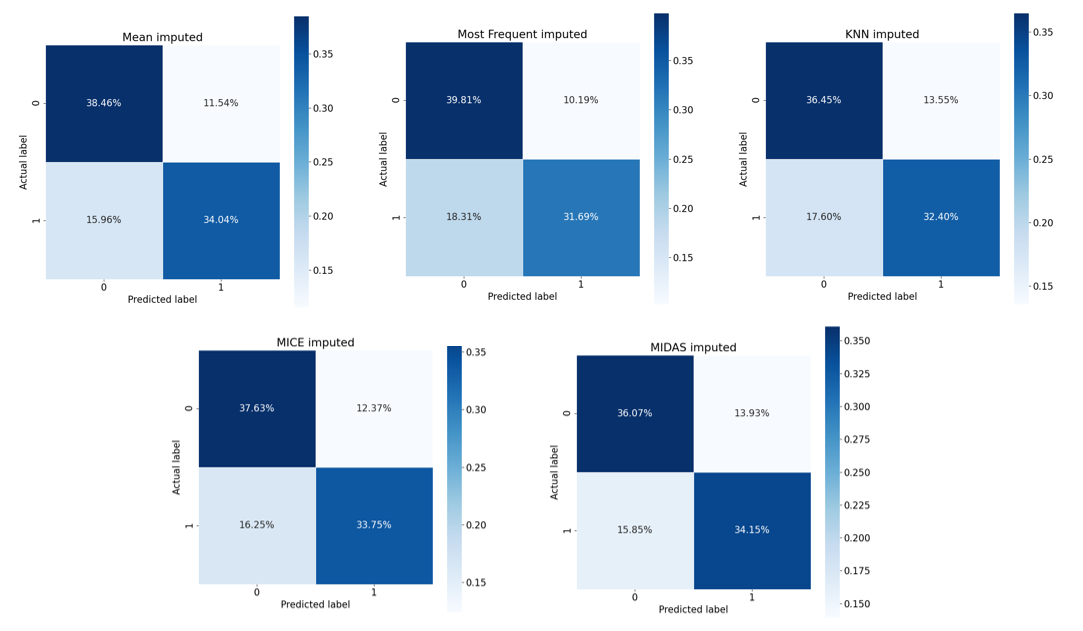
\includegraphics[width=\textwidth]{dissertation/Latex/images/Classification Results/lg_cm.PNG}
\end{figure}

 Looking at the confusion matrix in figure 6.8, we could see the that the model are making similar amount of predictions for both classes and is not over-fitted to either classes after applying under sample majority to our imputed dataset. Despite the huge decrease in accuracy without under sample majority, it was only predicting 0 since most of patients in the original training data was still alive after 48 hours. 

\subsection{Receiver Operating Characteristic (ROC) curve}

ROC curve is the plot of the false positive rate (x-axis) and true positive rate (y-axis). The curve visualises the balance between sensitivity (true positive rate) and specificity (true negative rate), which can also be represented by equation 6.5 and 6.6 respectively. Visually, the model is performing the best when it is closest to the top left corner of the graph. A random classifier by chance is represented as a diagonal line in ROC as a baseline, where the closer it gets to the 45 degree line, the less accurate the line. The area under curve (AUC) of the ROC curve is a Metric often used with ROC curves to measure how well a model is capable of distinguishing between classes. It can also be interpreted as the integral of the ROC curve from 0 to 1. The ROC curve is also often used in diagnostic testing and disease classification in medicine outside of machine learning, which makes this metric even more suitable for our clinical decision machine learning model. 

\begin{equation} \label{eq:5}
True positive rate = \frac{True Positives}{True Positive + False negative}
\end{equation}

\begin{equation} \label{eq:6}
False positive rate = \frac{False Positives}{False Positive + True negative}
\end{equation}

 \begin{figure}[!htb]
  \caption{Logistic Regression 5 Cross Validation ROC-Curves}
  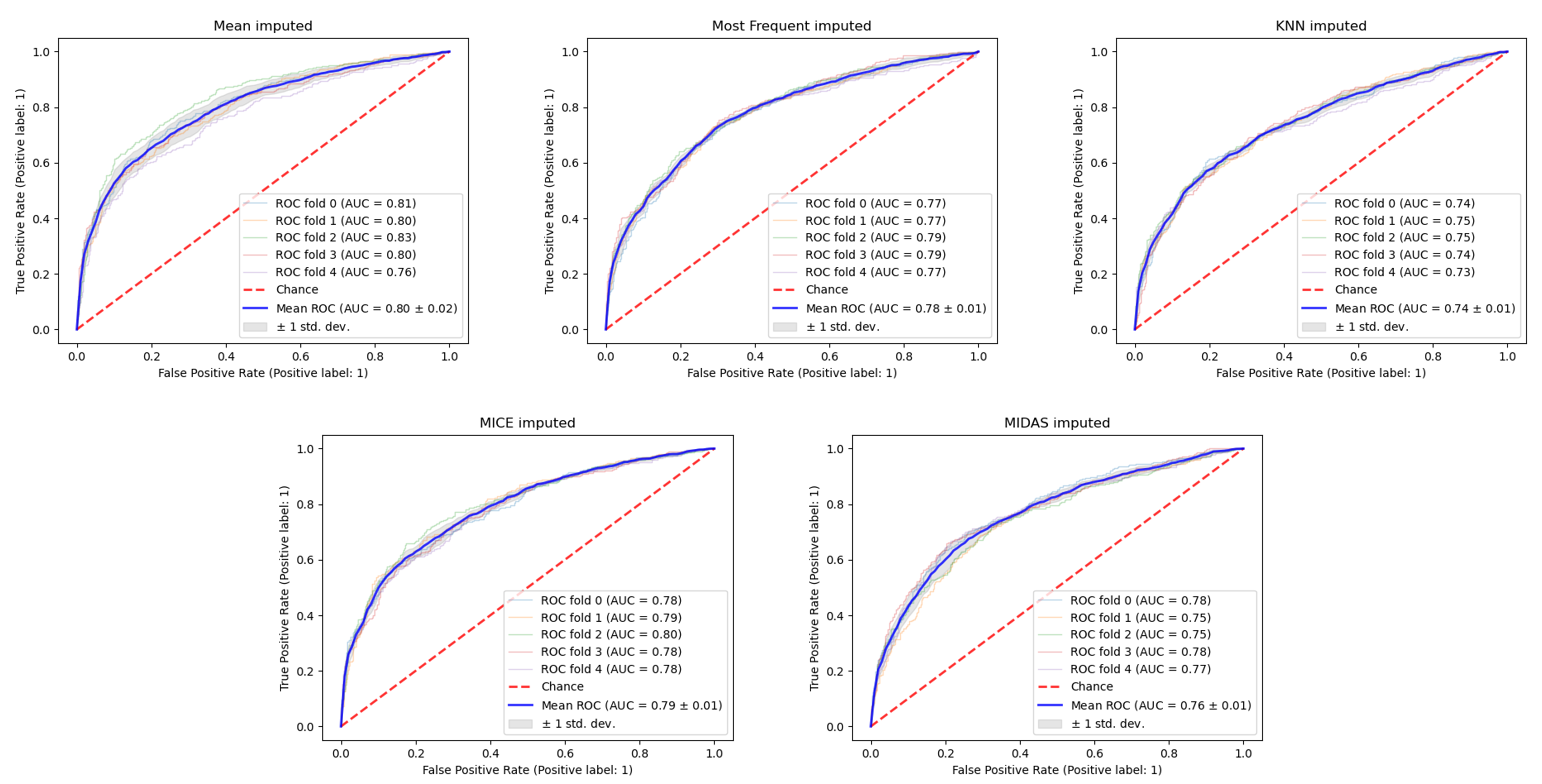
\includegraphics[width=\textwidth]{dissertation/Latex/images/Classification Results/lg_roc.PNG}
\end{figure}

 \begin{figure}[!htb]
  \caption{Random Forest 5 Cross Validation ROC-Curves}
  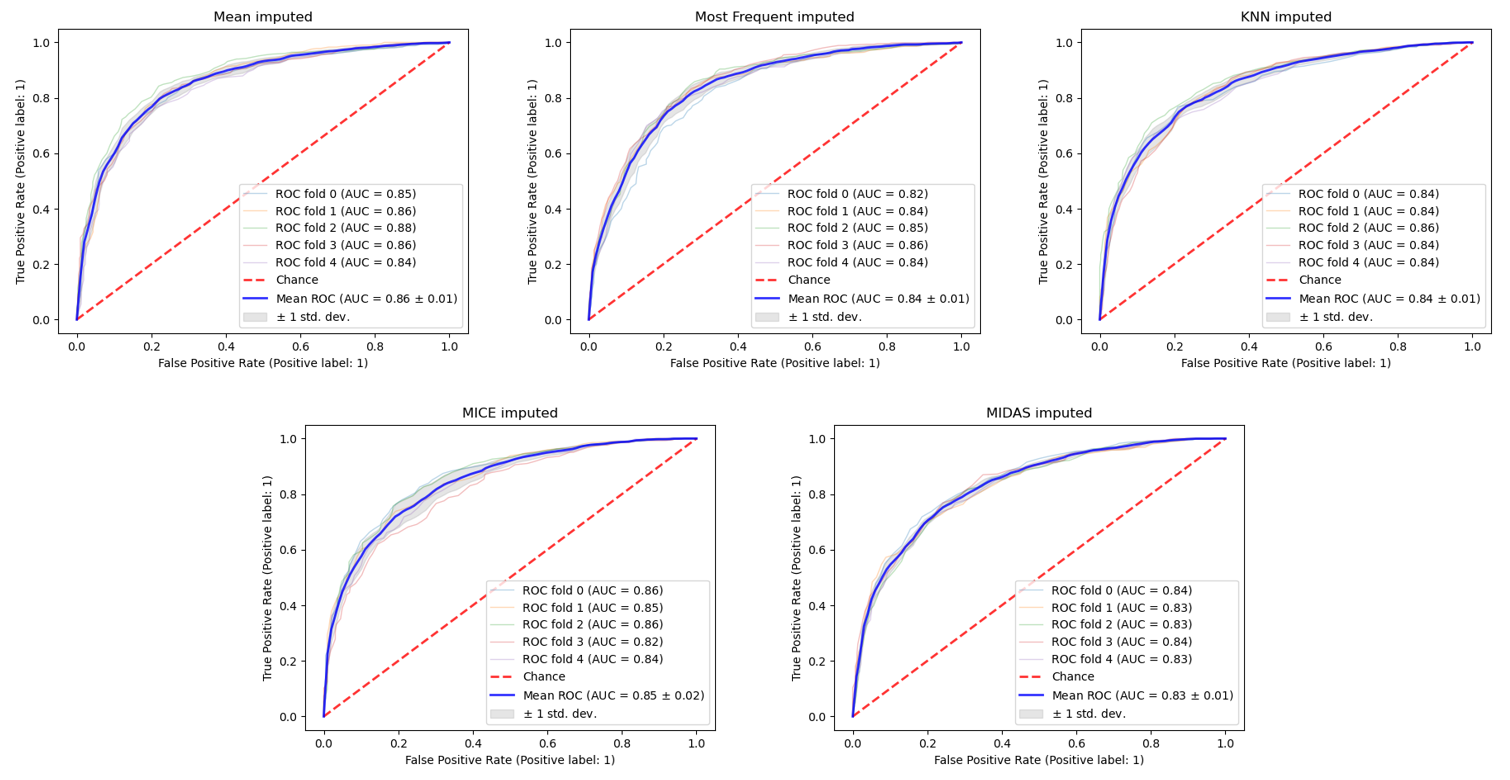
\includegraphics[width=\textwidth]{dissertation/Latex/images/Classification Results/rf_roc.PNG}
\end{figure}

Comparing the ROC curves and AUC of each imputation strategy for logistic regression in figure 6.9, we see that Mean imputed performed slightly better by 0.01 with a score of 0.80 followed by MICE imputation and Most frequent imputation. We also see a similar trend for random forest where mean imputed performed 0.01 better than MICE imputed with a higher score of 0.86. Overall, we can conclude that the difference in ROC and AUC is small and  statistically insignificant after applying the Friedman test hypothesis testing technique similar to f1-score. Which further backs up the previous hypothesis of the different imputation strategy being statistically insignificant.


\subsection{Permutation Feature importance}

Since logistic regression had a statistically significant difference in f1-scores for hypothesis testing, it might be useful to evaluate how important each medical variable is to the machine learning model using permutation feature importance. Permutation feature importance is a model inspection technique that can be used to analyse the weights and importance of the each features. Feature importance is defined to be the decrease in a model score when a single feature value is randomly shuffled, \cite{scikit-learn}. This procedure random shuffling breaks the relationship between the feature and target, and by tracking the drop in model score, we can quantify how much the model depends on the current feature. This 

 \begin{figure}[!htb]
  \caption{Logistic Regression Permutation Feature Importance }
  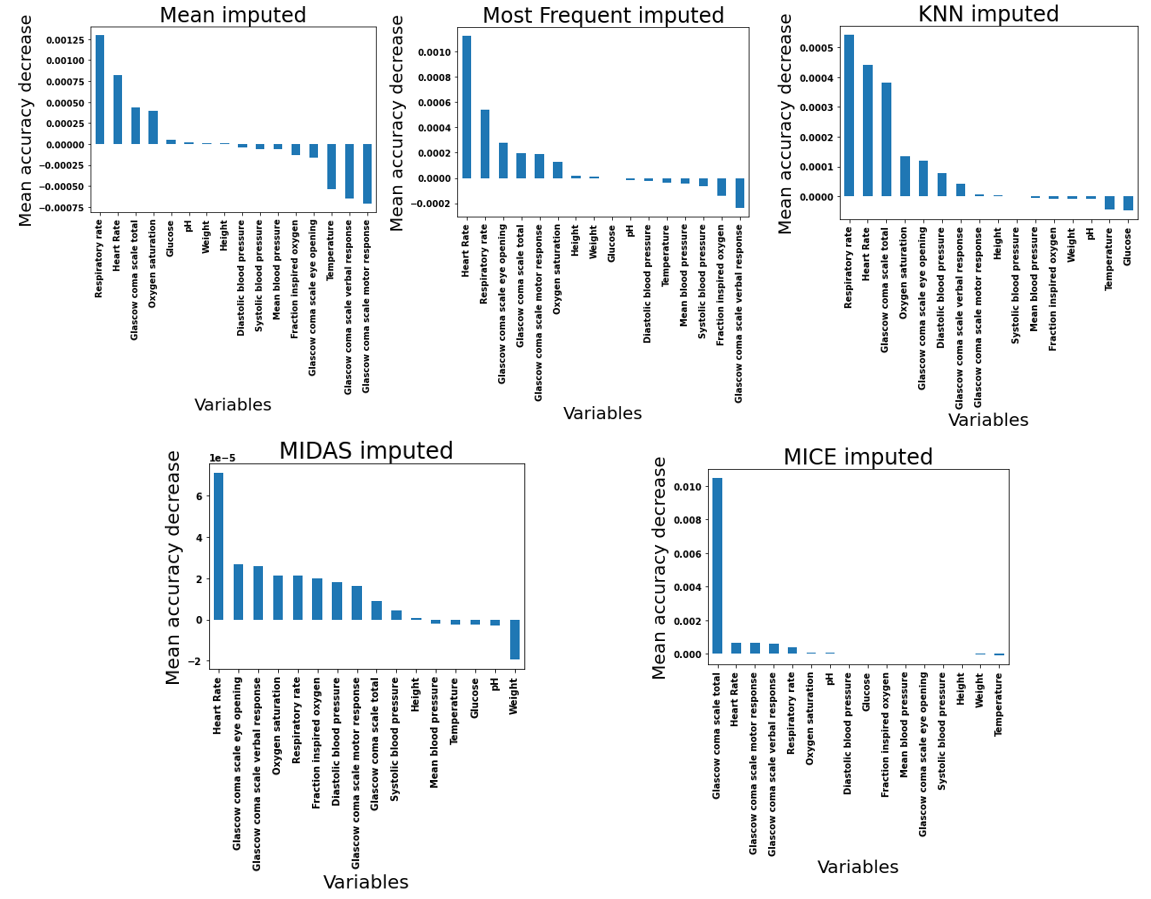
\includegraphics[width=\textwidth]{dissertation/Latex/images/Classification Results/lg_feature_importance.PNG}
\end{figure}


Looking at the feature importance diagram, it is interesting to see Glasgow coma variables to be least important for univariate strategies compared to the multivariate strategies. Glasgow coma scores are a measure of responsiveness and is often used to track level of consciousness after a brain injury, the lower the score, the lower the consciousness. This suggest the patients with record of this score had some consciousness related injury, and is more likely to have a lower score compared to other patients in the dataset with a missing value in this variable. Taking the mean of the score for these patients that is likely to have consciousness issues and using that value to impute other patients will create a biased score that is probably higher than the actual score. While for multivariate imputation strategies like MICE, it considers all other features during imputation, therefore we could see that there are significantly less variables that negatively affect the machine learning model. 

\section{Failed experiments}
Since this machine learning task involves time series data, the concept of time-since-measured was originally hypothesised to affect the machine learning performance, where aggregate function for count is used to keep track of the time since measured between all variables. However, after thorough testing using cross validation and hypothesis testing, it was proven to be statistically insignificant which was therefore removed from the final implementation.

Effort was also given into doing feature selection as a pre-processing step for the clinical decision system. This was achieved by using Principle component analysis and recursive feature elimination. However both feature selection method did not proof to improve the overall results significant, which was therefore not used for the final implementation. 

Deep learning classification using long short term memory (LSTM) and autoencoders was originally used for in-hospital mortality classification. However, the performance of these models is similar and sometimes worse than the classical machine learning models used. Since a lot of experiments and iterations is needed to evaluate the imputation strategies, the long run time of deep learning models was excessive and also does not contribute to the research question of investigating imputation strategies.



%==================================================================================================================================
\chapter{Discussion and Conclusion}    

\section{Summary}

Solving the problem of missing data in electronic health record was a challenging and ambiguous task. This is mostly due to the large amount of missing data to begin with and complex relationships between different variables that is difficult to learn for deep learning. After analysing the missingness of the MIMIC dataset and exploring feature importance in our models, it is concluded that uni-variate strategies like mean imputation is not suitable as imputation strategies for medical data. The main reason being the large amount of bias introduced and the ignored inherit uncertainty of missing values. Despite the decent performance when used to create risk prediction models, the validation and testing became untruthful due to the natural bias introduced to the entire dataset.

In this study, we investigated state-of-the-art multi-variate imputation strategies alongside uni-variate strategies as baseline to impute missing data in electronic health records. Each method is evaluated in two different aspect, how similar is the imputed dataset compared to the original dataset, and how effective was the clinical decision model created using different imputed dataset. We concluded that Multiple Imputation by Chained Equations (MICE) was most capable of imputing data that closely resembles the original data both in terms of Root Mean Squared Error (RMSE) in the holdout value simulation (Section 6.3) and by analysing the distribution of the original data (Section 6.2). In terms of performance for the in-hospital mortality prediction model, Although the clinical decision model created using MICE imputation was in general the best performing model. However it was concluded after in-depth statistical analysis of f1-score and ROC AUC score (Section 6.4) that the difference in performance for different imputation strategies is statistically insignificant. This might be due the the limited cross-validations fold or the limited amount of clinical data. Despite the statistical insignificant performance, it is concluded that MICE imputation is the most all-rounded imputation strategy and most suitable for imputation with Electronic health records and clinical researches. Although Deep learning imputation strategies has the potential to be the prefered method in the future, it is still in an early phase and not very trusted.

\section{Limitations and Future Work}

The biggest problem faced out of all was the problem with computational time. Despite there being a lot of missing values, the dataset is still extremely large, which makes slow algorithm like KNN and more complex algorithms like MIDAS to have even longer run times. For example, a single imputation run for KNN on the dataset took near 21 hours to compute, and the MIDAS model taking around 4 hours with just 25 iterations. This greatly discouraged hyper-paramter tuning and even affected the leave one out cross validation (LOOCV) experiment, since the number of folds for cross validation was lowered to 3 due to extremly long run times. Evaluation measures like coverage rate and average width was also not possible since the results are not representative with too little folds. 

In the current extraction pipeline, only 16 baseline variables are selected from the mimic dataset. More variables was not introduced in this research hugely due to the limitations to run time and the increased complexity to the pre-processing stages. If time allow, introducing more variables could very possibly improve the clinical decision model performance and also possibly the effectiveness of multi-variate imputation strategies.

Another natural challenge of working with medical data is the problem of class imbalance. When classifying in-hospital mortality, it is only normal to have more survivors than causalities in the hospital data. However, having too much data of the same class will often cause over-fitting and make the machine learning model meaningless where it only predicts one class. Although pre-processing methods like under-sampling and oversampling could help to solve this problem, these method greatly reduces the amount of training data. The obvious solution to this problem is to gather more data to begin with. As the MIMIC-Database continue to grow in size with future releases, there will be more and more data to work with and would probably allow more accurate imputation and clincial decision models. 

Granting that the amount of data in a clinical database is important, the quality of these data is just as important. If more data is introduced but these data includes just as much missing data, it would not be meaningful data and could possibly introduce more bias due to more missingness. Future work to gather more complete and consistent medical recordings in future releases of clinical database would greatly affect and benefit the field of research for clinical decision machine learning models.

For the deep learning imputation method MIDAS, the original plan was the create an original deep learning imputation method for this research. However, with limited knowledge in deep learning to begin with, it was a task too ambiguous to begin given limited time and resources to work on this project. However, even using the MIDAS library was exceptionally time consuming due to the complex theory behind it's implementation, and with limited support in optimizing this library, it was difficult to make MIDAS algorithm work as good as it's research paper by \cite{lall_robinson_2022} suggested. Future work on optimizing the model and with more computational resources, this imputation method as the potential to be significantly better than all imputations strategies explored in this project.

It was an a challenging, but interesting research for someone with no medicine related knowledge and limited experience in machine learning and deep learning. Learning to handle complex data-set and applying extraction pipelines was also difficult due to the natural complexity of the clinical dataset and medical research field. However, it was exiting to explore these new concepts and I have learnt more from this project than any other courses. If the quality and size of clinical databases continue to grow, I believe the research in using machine learning and artificial intelligence for clinical decision support system will surely revolutionize the medical industry in the near future.



%==================================================================================================================================
%
% 
%==================================================================================================================================
%  APPENDICES  

\begin{appendices}

\chapter{Appendices}

\section{Ethics course certificate}
\label{appendix:certificate}

\includegraphics[width=\textwidth]{dissertation/Latex/images/citiCompletionReport10596230 (1).PNG}
\pagebreak

\section{SQL queries used in extraction pipeline}
\subsection{SQL query for extracting patients data}
\label{appendix:patientsSQL}
\begin{lstlisting}[language=SQL]https://www.overleaf.com/project/61cdf40559960869dd952453
with patient_and_icustay_details as (
    SELECT distinct
        p.gender, p.dob, p.dod, s.*, a.admittime, a.dischtime, a.deathtime, a.ethnicity, a.diagnosis,
        DENSE_RANK() OVER (PARTITION BY a.subject_id ORDER BY a.admittime) AS hospstay_seq,
        DENSE_RANK() OVER (PARTITION BY s.hadm_id ORDER BY s.intime) AS icustay_seq,
        DATE_PART('year', s.intime) - DATE_PART('year', p.dob) as admission_age,
        DATE_PART('day', s.outtime - s.intime) as los_icu
    FROM patients p 
        INNER JOIN icustays s ON p.subject_id = s.subject_id
        INNER JOIN admissions a ON s.hadm_id = a.hadm_id 
    WHERE s.first_careunit NOT like 'NICU'
        and s.hadm_id is not null and s.icustay_id is not null
        and (s.outtime >= (s.intime + interval '12 hours'))
        and (s.outtime <= (s.intime + interval '240 hours'))
    ORDER BY s.subject_id )
SELECT * 
FROM patient_and_icustay_details 
WHERE hospstay_seq = 1
    and icustay_seq = 1
    and admission_age >=  """ + str(min_age) + """
    and los_icu >= 0.5
    
\end{lstlisting}

\subsection{SQL query for extracting events data}
\label{appendix:eventsSQL}
\begin{lstlisting}[language=SQL]

SELECT c.subject_id, i.hadm_id, c.icustay_id, c.charttime, c.itemid, c.value, c.valueuom
FROM icustays i
INNER JOIN chartevents c ON i.icustay_id = c.icustay_id
where c.icustay_id in """ + str(icu_ids_to_keep) + """
  and c.itemid in """ + str(chartitems_to_keep) + """
  and c.charttime between intime and outtime
  and c.error is distinct from 1
  and c.valuenum is not null
UNION ALL
SELECT distinct i.subject_id, i.hadm_id, i.icustay_id, l.charttime, l.itemid, l.value, l.valueuom
FROM icustays i
INNER JOIN labevents l ON i.hadm_id = l.hadm_id
where i.icustay_id in """ + str(icu_ids_to_keep) + """
  and l.itemid in """ + str(labitems_to_keep) + """
  and l.charttime between (intime - interval '6' hour) and outtime
  and l.valuenum > 0 -- lab values cannot be 0 and cannot be negative
  
\end{lstlisting}


\section{Machine Learning Results}
\subsection{Logistic Regression}
\label{appendix:lgresults}
 \begin{figure}[!h]
  \caption{Logistic Regression 5 Cross Validation ROC-Curves}
  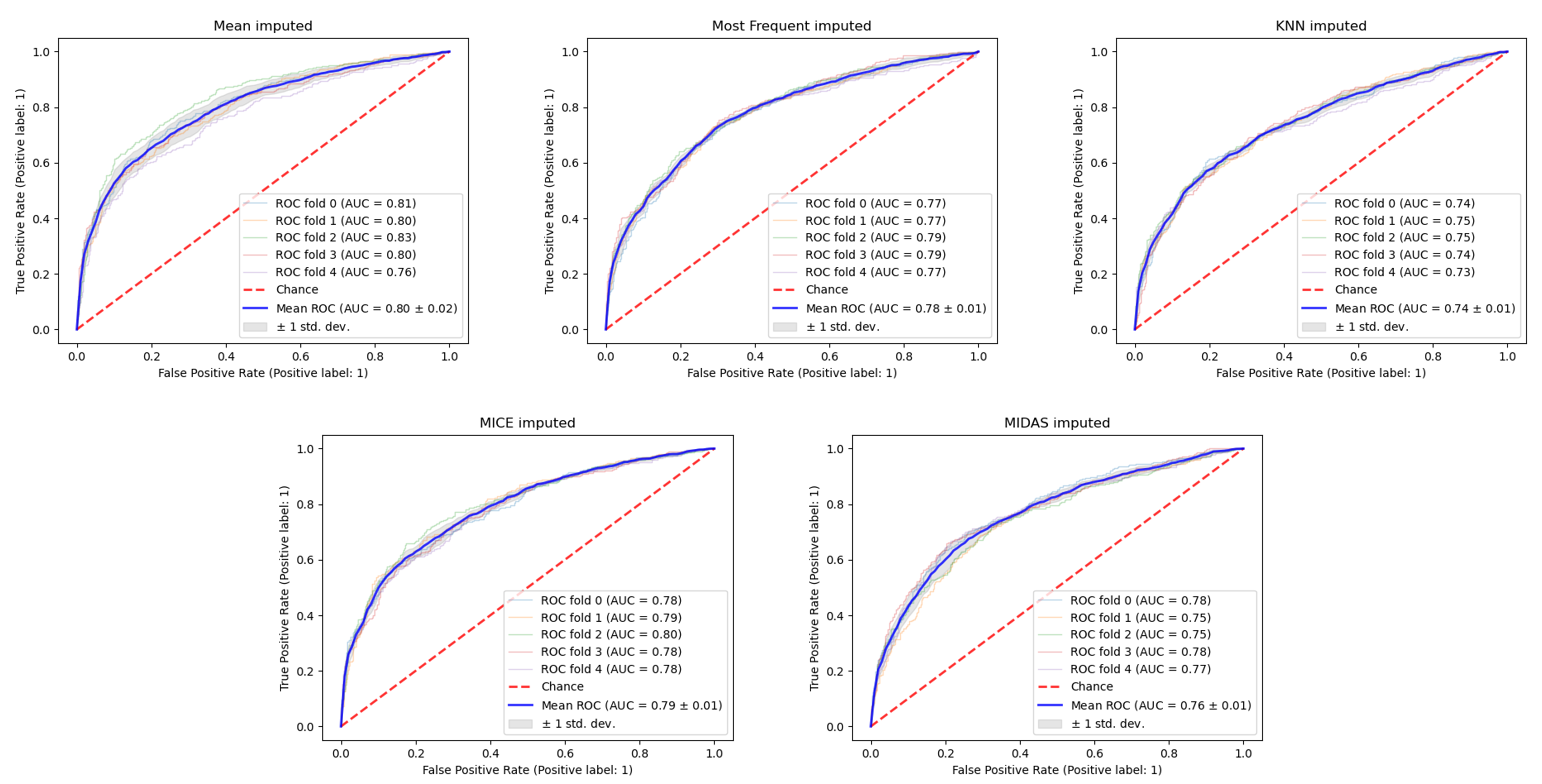
\includegraphics[width=\textwidth]{dissertation/Latex/images/Classification Results/lg_roc.PNG}
\end{figure}

\begin{figure}[!h]
  \caption{Logistic Regression Confusion Matrix}
  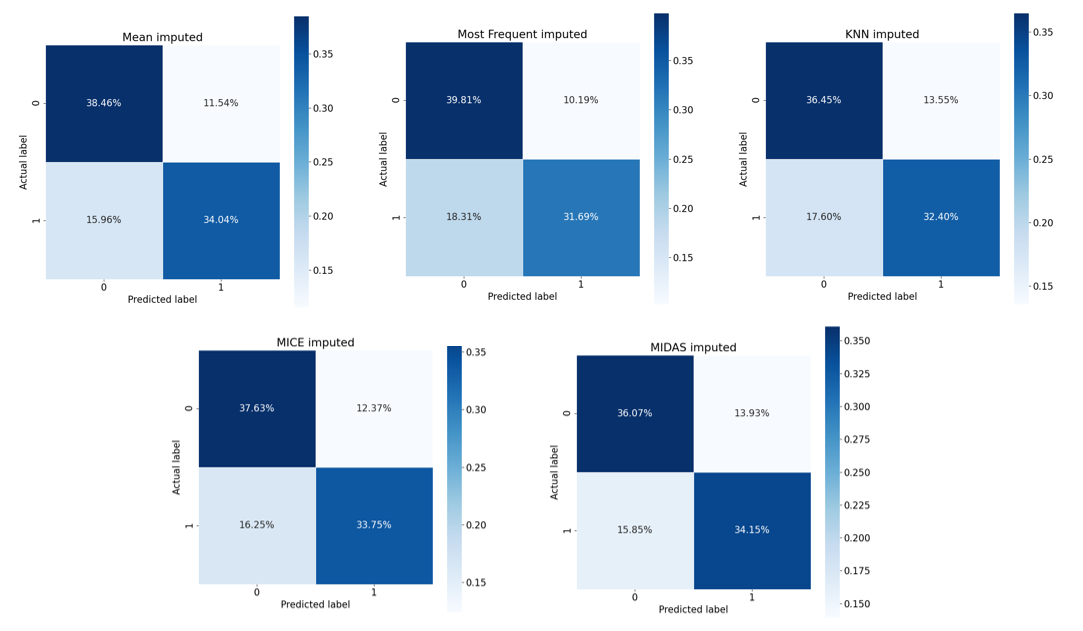
\includegraphics[width=\textwidth]{dissertation/Latex/images/Classification Results/lg_cm.PNG}
\end{figure}
\pagebreak

\subsection{Random Forest}
\label{appendix:rfresults}
 \begin{figure}[!h]
  \caption{Random Forest 5 Cross Validation ROC-Curves}
  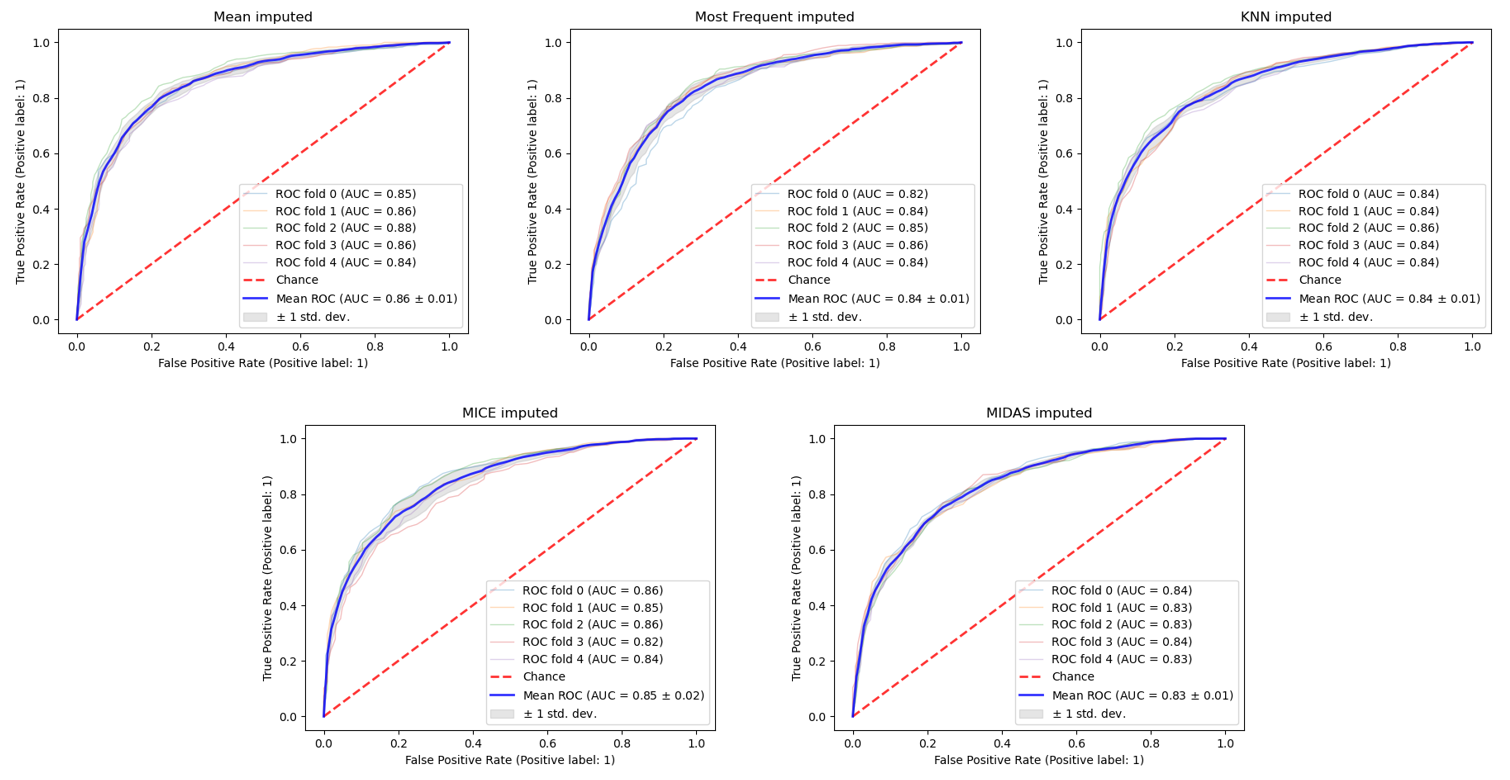
\includegraphics[width=\textwidth]{dissertation/Latex/images/Classification Results/rf_roc.PNG}
\end{figure}

\begin{figure}[!h]
  \caption{Random Forest Confusion Matrix}
  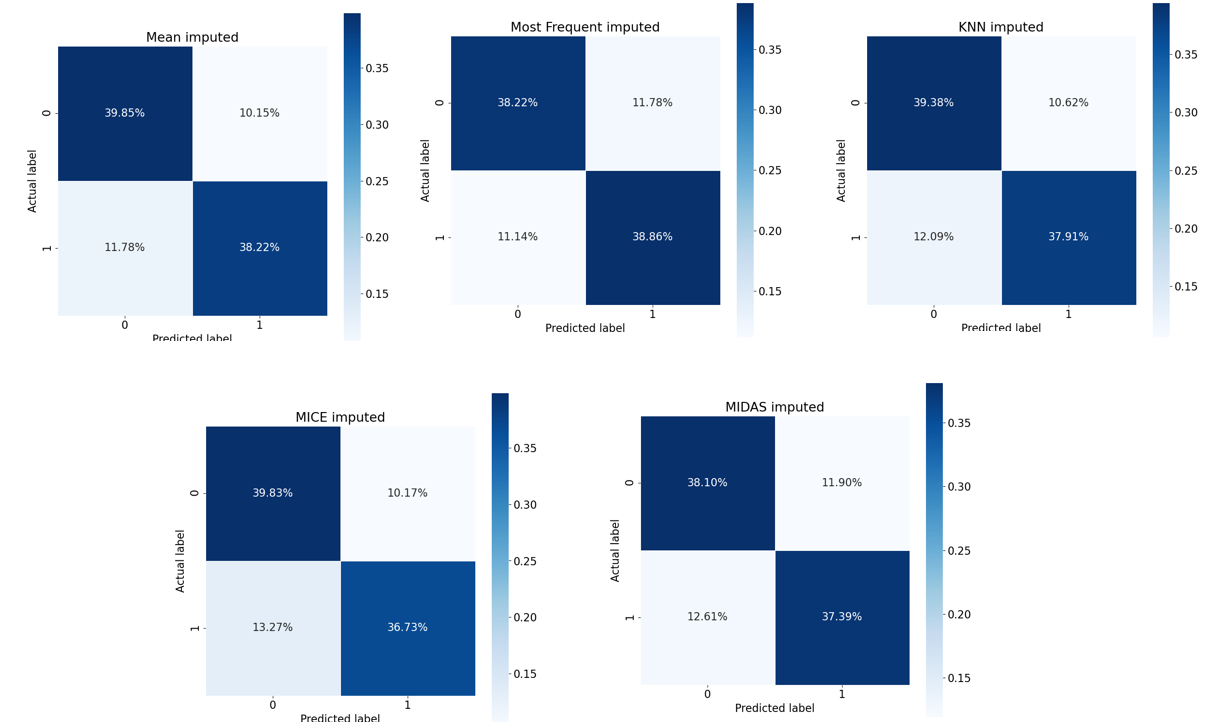
\includegraphics[width=\textwidth]{dissertation/Latex/images/Classification Results/rf_cm.PNG}
\end{figure}

\pagebreak
\subsection{Support Vector Classifier}
\label{appendix:svcresults}
 \begin{figure}[!h]
  \caption{Support Vector Classifier 5 Cross Validation ROC-Curves}
  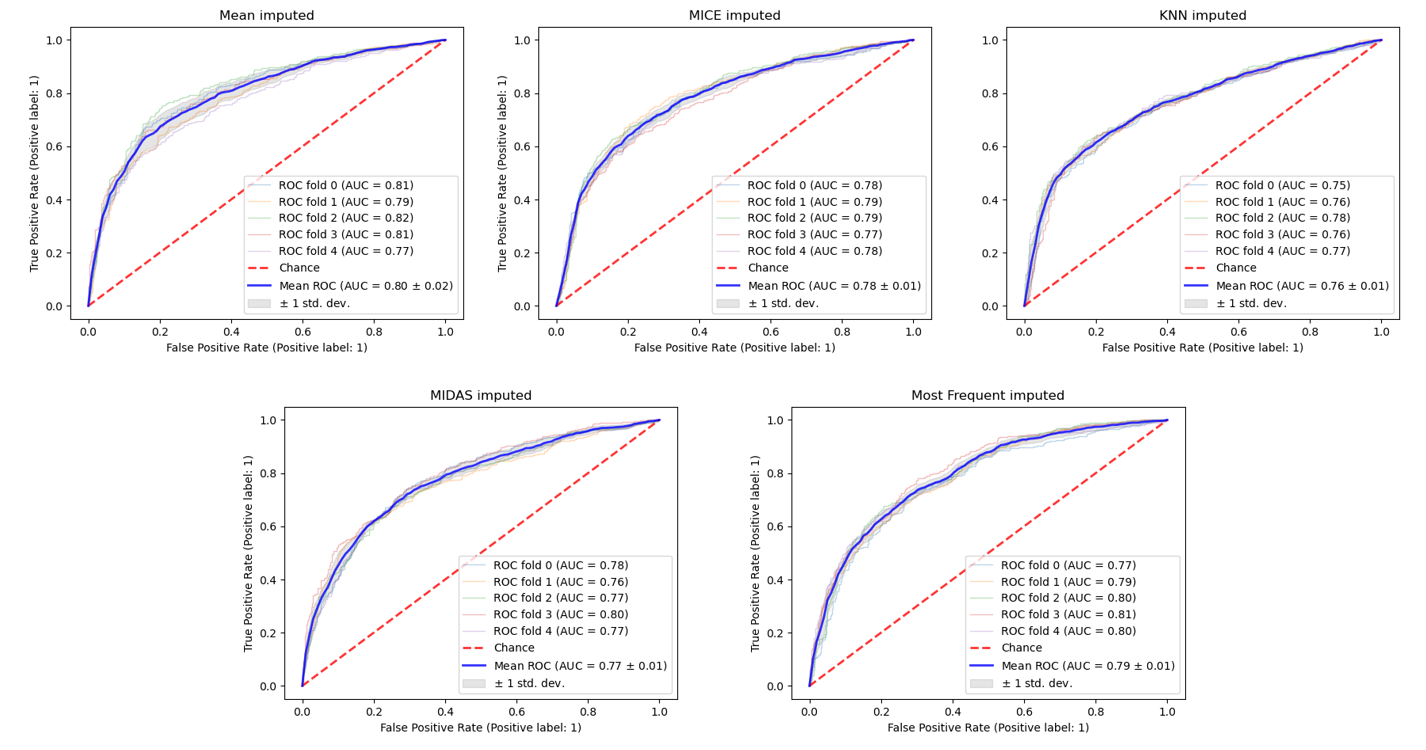
\includegraphics[width=\textwidth]{dissertation/Latex/images/Classification Results/svm_roc.PNG}
\end{figure}

\begin{figure}[!h]
  \caption{Support Vector Classifier Confusion Matrix}
  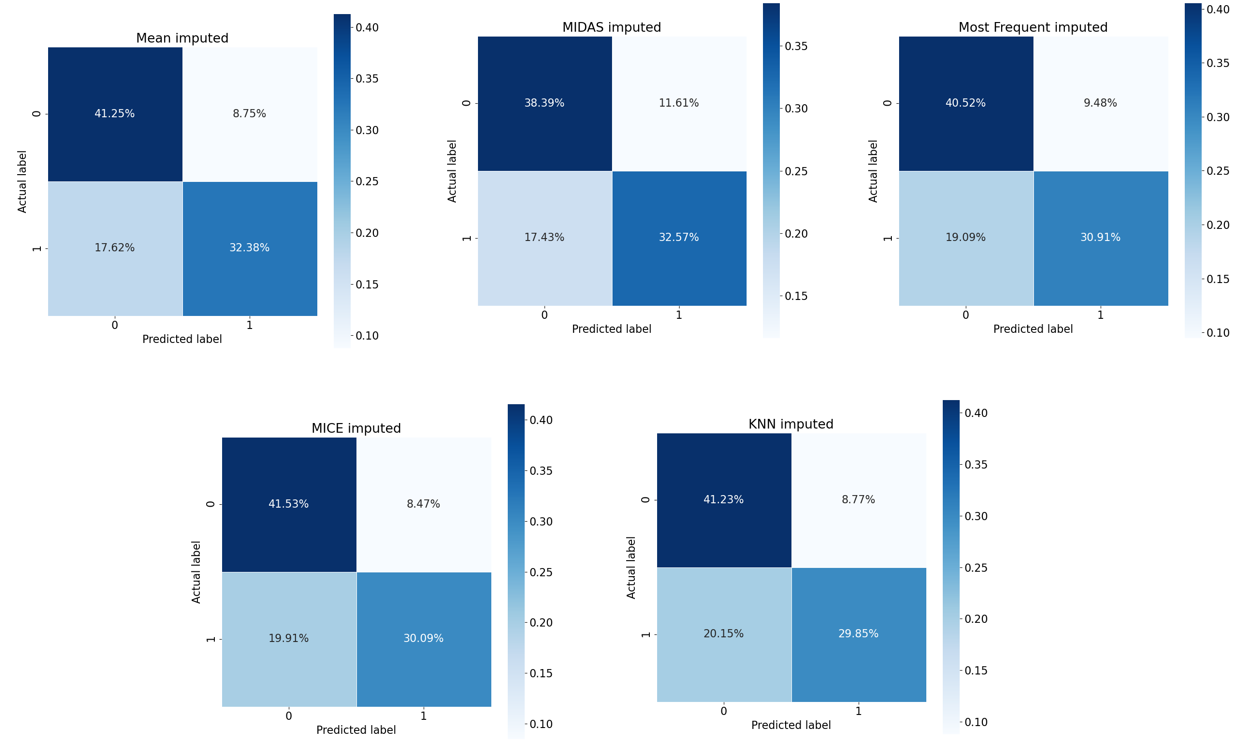
\includegraphics[width=\textwidth]{dissertation/Latex/images/Classification Results/svm_cm.PNG}
\end{figure}
\pagebreak

\section{Distributions graphs for all columns}
\label{appendix:distributions}
 \begin{figure}[!h]
  \caption{Imputed Data distributions for all medical variables}
  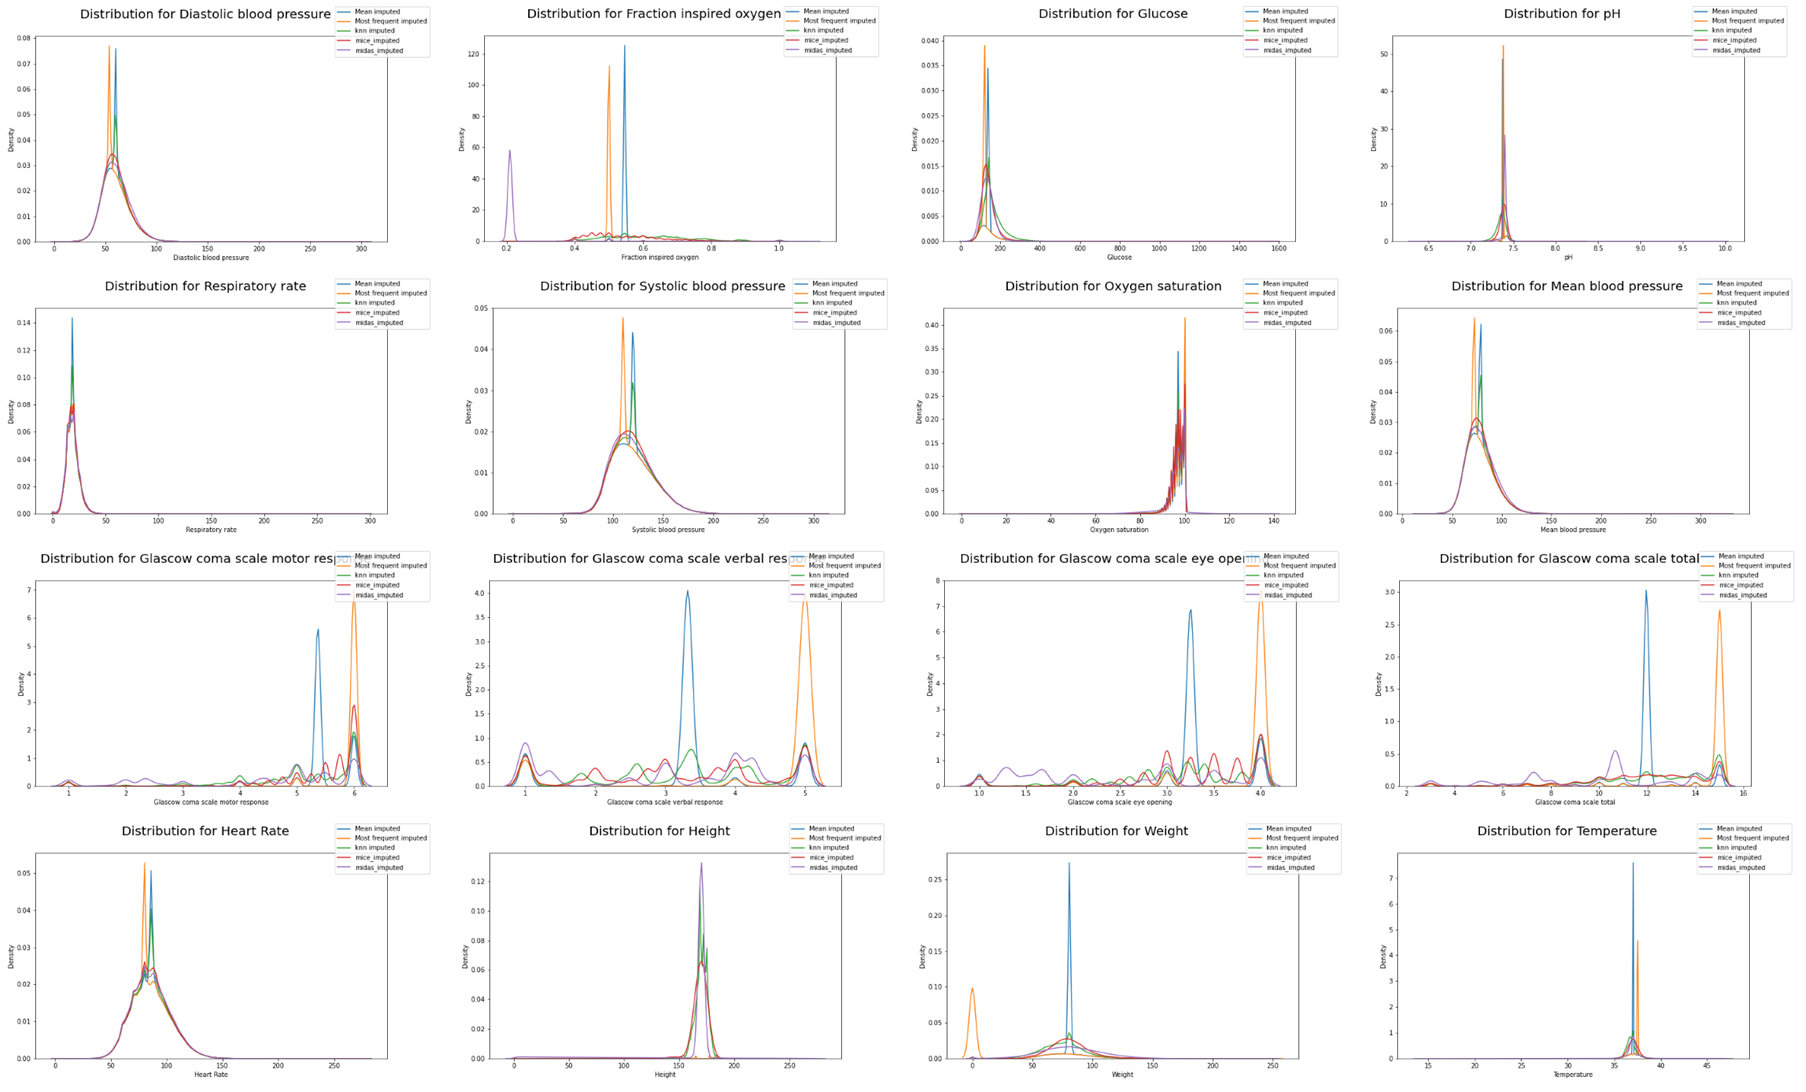
\includegraphics[width=\textwidth]{dissertation/Latex/images/distributions.PNG}
\end{figure}






\end{appendices}

%==================================================================================================================================
%   BIBLIOGRAPHY   

% The bibliography style is abbrvnat
% The bibliography always appears last, after the appendices.

\bibliographystyle{abbrvnat}

\bibliography{l4proj}

\end{document}
